% rubber: synctex
\documentclass{beamer}

\usepackage{amsmath,amsfonts}
\usepackage{bm}
\usepackage{nicefrac}
\usepackage{mathrsfs}
\usepackage{etex}
\usepackage{ccicons}
\usepackage{pgfplots,tikz}
\usepackage{tikz-qtree}
\usepackage{algorithms/algorithm}
\usepackage{algorithms/algorithmic}
\usepackage[T1]{fontenc}
\usepackage{cancel}
\usepackage{xcolor}
\usepackage{rotating}


\newlength\figureheight
\newlength\figurewidth

\definecolor{gray}{gray}{0.4}

\makeatletter
\@ifclassloaded{beamer}{
\usefonttheme[onlymath]{serif}
\uselanguage{French}
\languagepath{French}
% Git hash
\usepackage{xstring}
\usepackage{catchfile}
\immediate\write18{git rev-parse HEAD > git.hash}
\CatchFileDef{\HEAD}{git.hash}{\endlinechar=-1}
\newcommand{\gitrevision}{\StrLeft{\HEAD}{7}}
}{}
\makeatother

\makeatletter
\@ifclassloaded{beamer}{
\setbeamertemplate{footline}{
  {\hfill\vspace*{1pt}\href{https://creativecommons.org/publicdomain/zero/1.0/legalcode.en}{\ccZero}\hspace{.1cm}
    \href{https://mnemosyne.ithaca.fr/stephane/ep-mj-30-years/blob/\HEAD/tex/slides/sep.tex}{\gitrevision}\enspace--\enspace\today\enspace
  }}}
\makeatother

\makeatletter
\newenvironment{sqcases}{%
  \matrix@check\sqcases\env@sqcases
}{%
  \endarray\right.%
}
\def\env@sqcases{%
  \let\@ifnextchar\new@ifnextchar
  \left\lbrack
  \def\arraystretch{1.2}%
  \array{@{}l@{\quad}l@{}}%
}
\makeatother


\begin{document}

\setbeamertemplate{navigation symbols}{}

\pgfplotsset{every tick label/.append style={font=\tiny}}

\title{The stochastic extended path approach}
\author{St\'ephane Adjemian\footnote{Universit\'e du Mans, Dynare team} and Michel Juillard\footnote{Dynare team}}
\date{February, 2025}

\begin{frame}
   \titlepage{}
\end{frame}


\begin{frame}
   \frametitle{Motivations}

   \begin{itemize}

      \item Nonlinearities can play an important role in macroeconomics:
            Irreversible investment, ZLB, Borrowing constraint, \ldots\newline

      \item Standard local approximation techniques fail to produce
            reliable results in the presence of kinks.\newline

      \item Deterministic, perfect forresight models can be solved with much
            greater accuracy than stochastic ones.\newline

      \item The extended path approach aims to leverage the accuracy of
            deterministic methods in capturing (deterministic) nonlinearities.\newline

      \item But it neglects the implications of future uncertainty. Is
            this a concern? Can we improve the EP approach?

   \end{itemize}
\end{frame}


\begin{frame}
   \frametitle{Model to be solved}

   \[
      \mathbb E_t\left[ f\left( y_{t-1},y_t,y_{t+1},\varepsilon_t \right) \right] = 0
   \]

   \bigskip

   \begin{itemize}

      \item $y$ an $n\times 1$ vector of endogenous variables\newline

      \item $f: \mathbb R^{3n+q}\rightarrow \mathbb R^n$\newline

      \item $\varepsilon_t \sim \mathcal N\left( 0,\Sigma \right) \perp y_{\underline{t-1}}$\newline

      \item $ \exists\, y^{\star}$ such that $f\left( y^{\star},y^{\star},y^{\star},0 \right)=0$

   \end{itemize}

\end{frame}


\begin{frame}
   \frametitle{Perfect foresight version}

   \[
      \begin{cases}
         f\left( {\color{red}y_{t-1}},y_t,y_{t+1},\varepsilon_t \right) = 0     \\
         f\left( y_{t+h-1},y_{t+h},y_{t+h+1}, 0 \right) = 0\quad h=1,\ldots,H-2 \\
         f\left( y_{t+H-2},y_{t+H-1},{\color{red}y^{\star}}, 0 \right) = 0      \\
      \end{cases}
   \]
   \bigskip

   \begin{itemize}

      \item For a long enough simulation, one can consider that for all
            practical purpose the system is back to equilibrium in period $H$.\newline

      \item[$\Rightarrow$] Two value boundary problem with
            initial conditions for some variables (states) and
            terminal conditions for others (jumpings).\newline

      \item In practice, one can use a Newton method to solve the equations of
            the model stacked over all periods of the simulation.\newline

   \end{itemize}

\end{frame}


\begin{frame}
   \frametitle{Perfect foresight model solver}

   \begin{itemize}

      \item The unknowns:\newline
            \[
               Y_t = (y_t', y_{t+1}',\ldots,y_{t+H-1}')' \quad\text{ a }nH\times 1\text{ vector}
            \]

            \bigskip

      \item We can rewrite the system of equations as $F(Y)=0$, and solve it recursively:\newline

            \[
               Y_t^{(i+1)} = Y_t^{(i)} - J_F\left(Y_t^{(i)}\right)^{-1} F\left(Y_t^{(i)}\right)
            \]
            \medskip

      \item The jacobian $J_F$ is potentially very large but \textbf{sparse}.

   \end{itemize}

\end{frame}


\begin{frame}
   \frametitle{Stochastic perfect foresight model}
   \framesubtitle{Stacked jacobian, order=1, three nodes}
   \begin{center}
      \scalebox{.5}{
         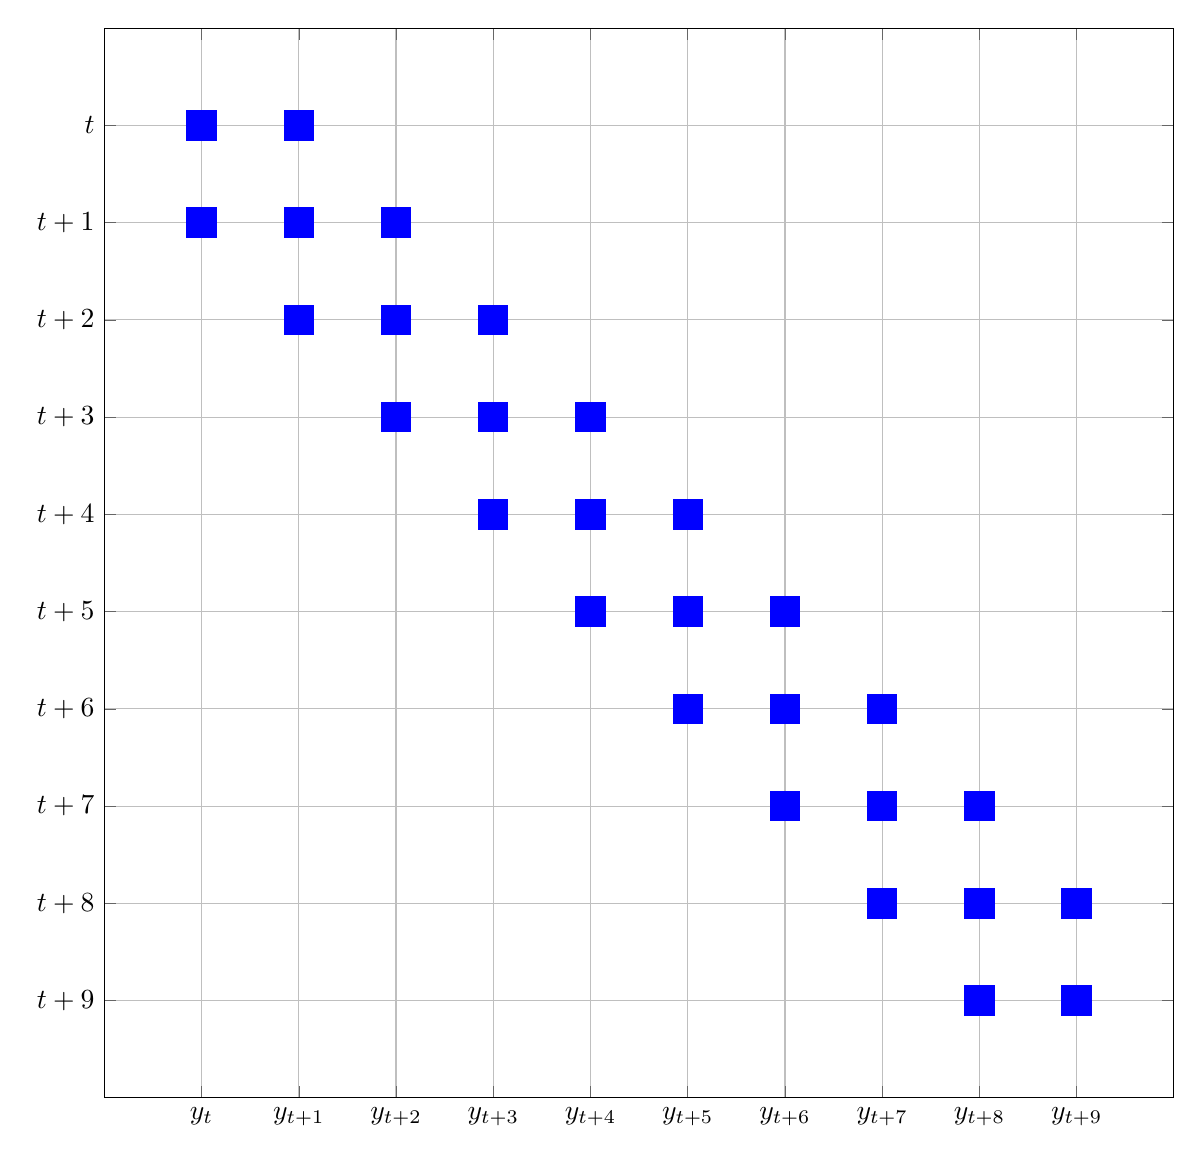
\begin{tikzpicture}

\begin{axis}[%
width=5.348in,
height=5.348in,
at={(1.854in,0.722in)},
scale only axis,
xmin=0,
xmax=11,
xtick={1,2,3,4,5,6,7,8,9,10},
xticklabels={{$y_t$},{$y_{t+1}$},{$y_{t+2}$},{$y_{t+3}$},{$y_{t+4}$},{$y_{t+5}$},{$y_{t+6}$},{$y_{t+7}$},{$y_{t+8}$},{$y_{t+9}$}},
y dir=reverse,
ymin=0,
ymax=11,
ytick={1,2,3,4,5,6,7,8,9,10},
yticklabels={{$t$},{$t+1$},{$t+2$},{$t+3$},{$t+4$},{$t+5$},{$t+6$},{$t+7$},{$t+8$},{$t+9$}},
axis background/.style={fill=white},
xmajorgrids,
ymajorgrids
]
\addplot [color=blue, only marks, mark size=5.3pt, mark=square*, mark options={solid, blue}, forget plot]
  table[row sep=crcr]
   \end{center}
\end{frame}


\begin{frame}
   \frametitle{Extended path}

   \begin{itemize}
      \item Unexpected shocks in each period\newline
      \item Loop over perfect foresight models\newline
   \end{itemize}

   \medskip

   \algsetup{
      linenosize=\small,
      linenodelimiter=.
   }
   \begin{algorithm}[H]
      \caption{Extended path algorithm}
      \label{alg:ep}
      \begin{algorithmic}[1]
         \STATE $H \leftarrow$ Set the horizon of the perfect foresight (PF) model.
         \STATE $y^\star \leftarrow$ Compute steady state of the model
         \STATE $y_{t-1} \leftarrow$ Choose an initial condition for the state variables
         \FOR{$\tau=t$ to $t+H-1$}
         \STATE $u_\tau  \leftarrow$ Draw random shocks for the current period
         \STATE $y_t \leftarrow$ Solve a PF with $y_{t+H}=y^{\star}$
         \ENDFOR
      \end{algorithmic}
   \end{algorithm}

\end{frame}


\begin{frame}
   \frametitle{Approximate expectation}

   \begin{itemize}
      \item Use gaussian quadrature
            \[
               \mathbb E \left[\varphi (X)\right] = \int \varphi(x)f(x)\mathrm dx \approx \sum_{i=1}^m \omega_i \varphi(x_i)
            \]
            where $(\omega_i,x_i)_{i=1}^m$ are the gaussian quadrature weight and nodes.\newline

      \item If more than one source of future uncertainty, use tensor product (default in Dynare).\newline

      \item[$\Rightarrow$] First curse of dimensionality.\newline

      \item Use unscented transform (Julier et at., 2000): number of nodes grows linearly w.r.t the number of shocks.

   \end{itemize}

\end{frame}


\begin{frame}[c]{}
   \frametitle{Tree of forward histories (second curse)}

   \begin{center}
      \begin{tikzpicture}[scale=.4]
         \tikzset{grow'=right,level distance=120pt}
         \tikzset{execute at begin node=\strut}
         \tikzset{every tree node/.style={anchor=base west}}
         \Tree [.$\varepsilon_t$
         [.$\epsilon_2$ [.$\epsilon_2$ \edge[dashed]; {} \edge[dashed]; {} \edge[dashed]; {} ]
         [.$\epsilon_1$ \edge[dashed]; {} \edge[dashed]; {} \edge[dashed]; {} ]
         [.$\epsilon_3$ \edge[dashed]; {} \edge[dashed]; {} \edge[dashed]; {} ]
         ]
         [.$\epsilon_1$ [.$\epsilon_2$ \edge[dashed]; {} \edge[dashed]; {} \edge[dashed]; {} ]
         [.$\epsilon_1$ \edge[dashed]; {} \edge[dashed]; {} \edge[dashed]; {} ]
         [.$\epsilon_3$ \edge[dashed]; {} \edge[dashed]; {} \edge[dashed]; {} ]
         ]
         [.$\epsilon_3$ [.$\epsilon_2$ \edge[dashed]; {} \edge[dashed]; {} \edge[dashed]; {} ]
         [.$\epsilon_1$ \edge[dashed]; {} \edge[dashed]; {} \edge[dashed]; {} ]
         [.$\epsilon_3$ \edge[dashed]; {} \edge[dashed]; {} \edge[dashed]; {} ]
         ]
         ]
      \end{tikzpicture}


   \end{center}
\end{frame}



\begin{frame}[c]{}
   \frametitle{Stochastic perfect foresight models}
   \framesubtitle{order 1}
   \centering
   \[
      \begin{split}
                                                                                & \sum_{i=1}^m\omega_i f\left( {\color{blue} y_{t-1}}, {\color{red} y_t}, y_{t+1}^i, \varepsilon_t\right) = 0                  \\
         \begin{sideways}\hspace{-.6cm}\footnotesize{i=1,\dots,m}\end{sideways} & \begin{sqcases}
                                                                                     f\left( {\color{red}y_t}, y_{t+1}^i, y_{t+2}^i, \epsilon_i \right) = 0\\
                                                                                     f\left( y_{t+1}^i, y_{t+2}^i, y_{t+3}^i, 0 \right) = 0\\
                                                                                     \vdots\\
                                                                                     f\left( y_{t+H-2}^i, y_{t+H-1}^i, {\color{blue}y^{\star}}, 0 \right) = 0\\
                                                                                  \end{sqcases}
      \end{split}
   \]

\end{frame}


\begin{frame}[c,fragile]{}
   \frametitle{Stochastic perfect foresight models}
   \framesubtitle{order 1}
   \centering

   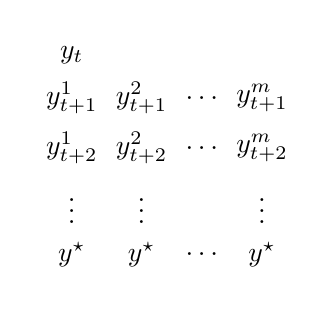
\begin{tikzpicture}
      \matrix
      {
         \node {$y_t$};                              & \node{};                                   & \node {};        & \node {};                                  \\
         \node {$y_{t+1}^1$};  & \node{$y_{t+1}^2$};  & \node{$\ldots$}; & \node{$y_{t+1}^m$};  \\
         \node {$y_{t+2}^1$}; & \node{$y_{t+2}^2$}; & \node{$\ldots$}; & \node{$y_{t+2}^m$}; \\
         \node {$\vdots$};                           & \node{$\vdots$};                           & \node{};         & \node{$\vdots$};                           \\
         \node {$y^\star$};                          & \node{$y^\star$};                          & \node{$\ldots$}; & \node{$y^\star$};                          \\
      };
   \end{tikzpicture}

   \bigskip\bigskip

   $\rightarrow\quad 1+m(H-1)$ unknown vectors ($n\times 1$).

\end{frame}



\begin{frame}
   \frametitle{Stochastic perfect foresight model}
   \framesubtitle{Stacked jacobian, order=1, three nodes}
   \begin{center}
      \scalebox{.5}{
         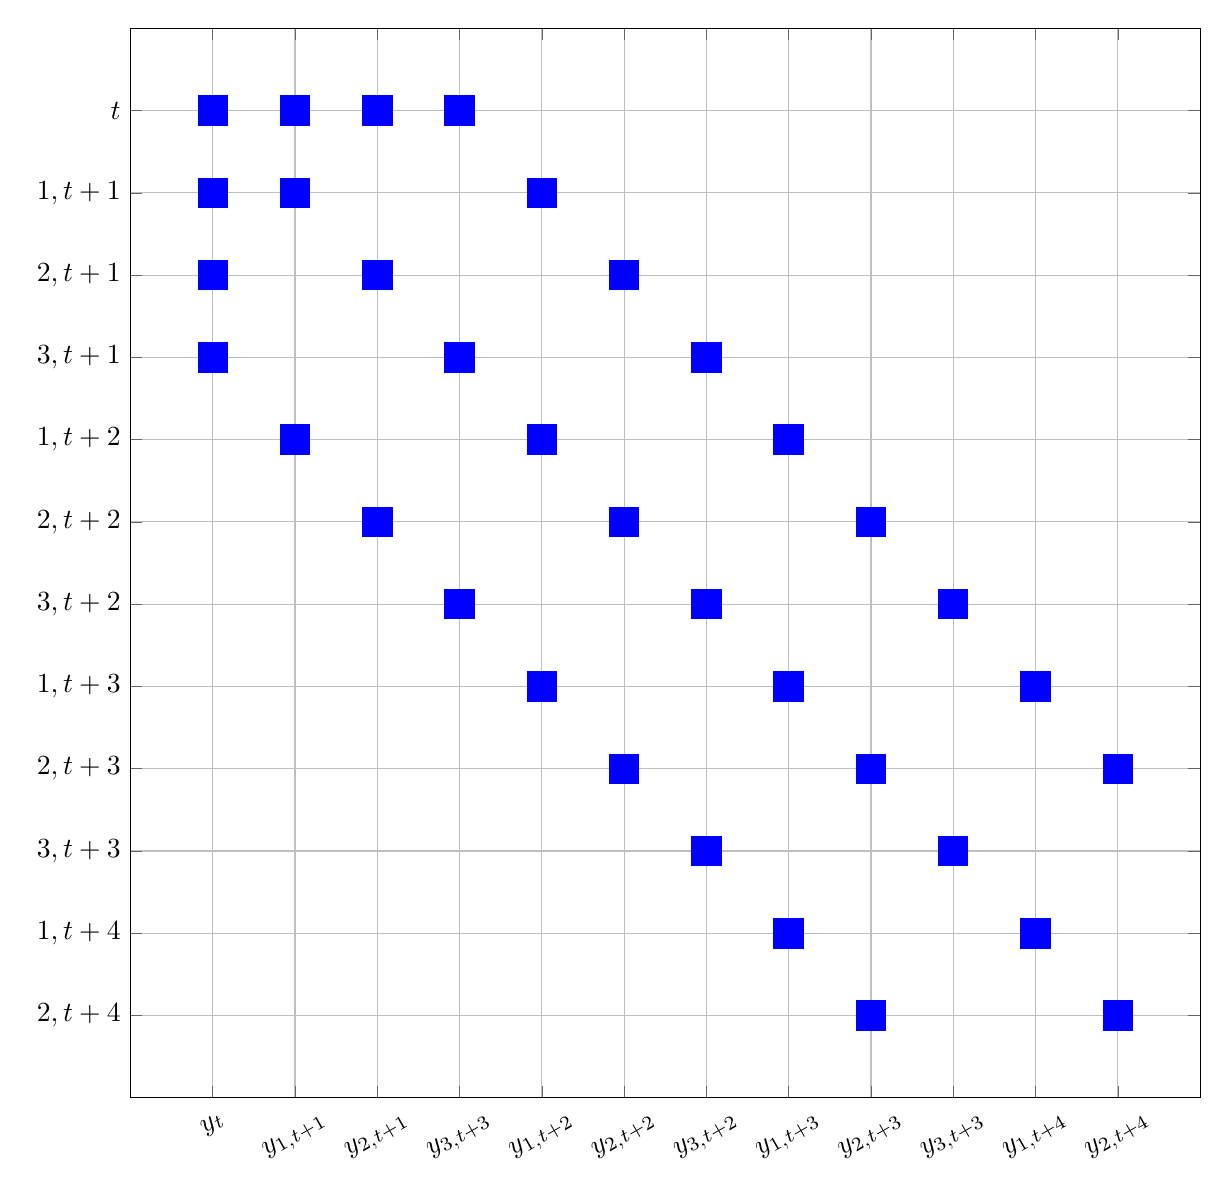
\begin{tikzpicture}

\begin{axis}[%
width=5.348in,
height=5.348in,
at={(1.854in,0.722in)},
scale only axis,
xmin=0,
xmax=13,
xtick={1,2,3,4,5,6,7,8,9,10,11,12},
xticklabels={$y_t$,$y_{1,t+1}$,$y_{2,t+1}$,$y_{3,t+3}$,$y_{1,t+2}$,$y_{2,t+2}$,$y_{3,t+2}$,$y_{1,t+3}$,$y_{2,t+3}$,$y_{3,t+3}$,$y_{1,t+4}$,$y_{2,t+4}$},
xticklabel style={rotate=30},
y dir=reverse,
ymin=0,
ymax=13,
ytick={1,2,3,4,5,6,7,8,9,10,11,12},
yticklabels={$t$,{$1,t+1$},{$2,t+1$},{$3,t+1$},{$1,t+2$},{$2,t+2$},{$3,t+2$},{$1,t+3$},{$2,t+3$},{$3,t+3$},{$1,t+4$},{$2,t+4$}},
axis background/.style={fill=white},
xmajorgrids,
ymajorgrids
]
\addplot [color=blue, only marks, mark size=5.3pt, mark=square*, mark options={solid, blue}, forget plot]
  table[row sep=crcr]
   \end{center}
\end{frame}


\begin{frame}[c]{}
   \frametitle{Stochastic perfect foresight models}
   \framesubtitle{order 2}
   \centering

   \[
      \begin{split}
                                                                                & \sum_{i=1}^m\omega_i f\left( {\color{blue} y_{t-1}}, {\color{red} y_t}, y_{t+1}^i, \varepsilon_t\right) = 0                \\
         \begin{sideways}\hspace{-.6cm}\footnotesize{i=1,\dots,m}\end{sideways} & \begin{sqcases}
                                                                                     \sum_{j=1}^m\omega_jf\left( {\color{red}y_t}, y_{t+1}^j, y_{t+2}^{j,i}, \epsilon_i \right) = 0\\
                                                                                     \begin{sideways}\hspace{-.6cm}\footnotesize{j=1,\dots,m}\end{sideways} \begin{sqcases}
               f\left( y_{t+1}^i, y_{t+2}^{j,i}, y_{t+3}^{j,i}, \epsilon_j \right) = 0\\
               f\left( y_{t+2}^{j,i}, y_{t+3}^{j,i}, y_{t+4}^{j,i}, 0 \right) = 0\\
               \vdots\\
               f\left(y_{t+H-2}^{j,i} , y_{t+H-1}^{j,i}, {\color{blue}y^{\star}}, 0 \right) = 0
            \end{sqcases}
                                                                                  \end{sqcases}
      \end{split}
   \]

\end{frame}


\begin{frame}[c,fragile]{}
   \frametitle{Stochastic perfect foresight models}
   \framesubtitle{order 2}
   \centering

   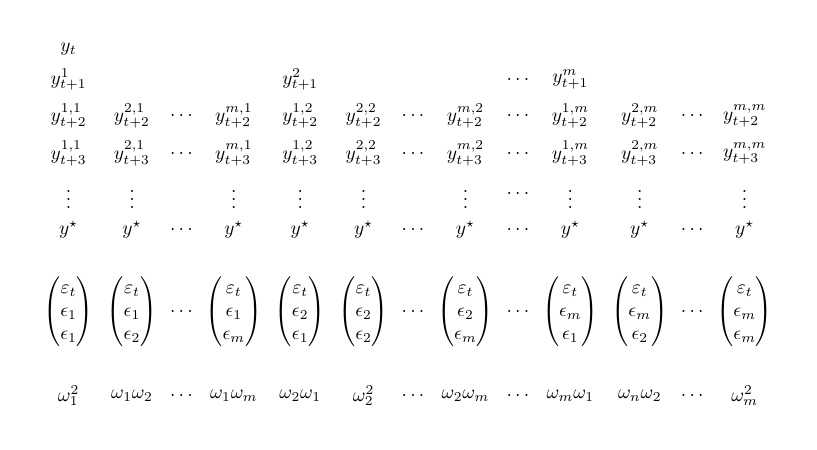
\begin{tikzpicture}[scale=0.7, every node/.style={scale=0.7}]
      \matrix
      {
         \node {$y_t$};                              & \node{};                                 & \node {};        & \node {}; \node {};                      & \node{};                                    & \node {};                                & \node {};        & \node{};                                 & \node{};         & \node {};                                   & \node {};                                & \node{};                                                    \\
         \node {$y_{t+1}^1$}; & \node{};                                 & \node{};         & \node{};                                 & \node {$y_{t+1}^2$}; & \node{};                                 & \node{};         & \node{};                                 & \node{$\ldots$}; & \node {$y_{t+1}^m$}; & \node{};                                 & \node{};         & \node{};                                 \\
         \node {$y_{t+2}^{1,1}$};   & \node{$y_{t+2}^{2,1}$}; & \node{$\ldots$}; & \node{$y_{t+2}^{m,1}$}; & \node {$y_{t+2}^{1,2}$};   & \node{$y_{t+2}^{2,2}$}; & \node{$\ldots$}; & \node{$y_{t+2}^{m,2}$}; & \node{$\ldots$}; & \node {$y_{t+2}^{1,m}$};   & \node{$y_{t+2}^{2,m}$}; & \node{$\ldots$}; & \node{$y_{t+2}^{m,m}$}; \\
         \node {$y_{t+3}^{1,1}$};   & \node{$y_{t+3}^{2,1}$}; & \node{$\ldots$}; & \node{$y_{t+3}^{m,1}$}; & \node {$y_{t+3}^{1,2}$};   & \node{$y_{t+3}^{2,2}$}; & \node{$\ldots$}; & \node{$y_{t+3}^{m,2}$}; & \node{$\ldots$}; & \node {$y_{t+3}^{1,m}$};   & \node{$y_{t+3}^{2,m}$}; & \node{$\ldots$}; & \node{$y_{t+3}^{m,m}$}; \\
         \node {$\vdots$};                           & \node{$\vdots$};                         & \node{};         & \node{$\vdots$};                         & \node {$\vdots$};                           & \node{$\vdots$};                         & \node{};         & \node{$\vdots$};                         & \node{$\ldots$}; & \node {$\vdots$};                           & \node{$\vdots$};                         & \node{};         & \node{$\vdots$};                         \\
         \node {$y^\star$};                          & \node{$y^\star$};                        & \node{$\ldots$}; & \node{$y^\star$};                        & \node {$y^\star$};                          & \node{$y^\star$};                        & \node{$\ldots$}; & \node{$y^\star$};                        & \node{$\ldots$}; & \node {$y^\star$};                          & \node{$y^\star$};                        & \node{$\ldots$}; & \node{$y^\star$};                        \\
         \node {};                                   & \node{};                                 & \node{};         & \node{};                                 & \node {};                                   & \node{};                                 & \node{};         & \node{};                                 & \node{};         & \node {};                                   & \node{};                                 & \node{};         & \node{};                                 \\
         \node {};                                   & \node{};                                 & \node{};         & \node{};                                 & \node {};                                   & \node{};                                 & \node{};         & \node{};                                 & \node{};         & \node {};                                   & \node{};                                 & \node{};         & \node{};                                 \\
         \node {$\begin{pmatrix}\varepsilon_t\\ \epsilon_1 \\ \epsilon_1\end{pmatrix}$};       & \node{$\begin{pmatrix}\varepsilon_t\\ \epsilon_1 \\ \epsilon_2\end{pmatrix}$};     & \node{$\ldots$}; & \node{$\begin{pmatrix}\varepsilon_t\\ \epsilon_1 \\ \epsilon_m\end{pmatrix}$};     & \node {$\begin{pmatrix}\varepsilon_t\\ \epsilon_2 \\ \epsilon_1\end{pmatrix}$};       & \node{$\begin{pmatrix}\varepsilon_t\\ \epsilon_2 \\ \epsilon_2\end{pmatrix}$};     & \node{$\ldots$}; & \node{$\begin{pmatrix}\varepsilon_t\\ \epsilon_2 \\ \epsilon_m\end{pmatrix}$};     & \node{$\ldots$}; & \node {$\begin{pmatrix}\varepsilon_t\\ \epsilon_m \\ \epsilon_1\end{pmatrix}$};       & \node{$\begin{pmatrix}\varepsilon_t\\ \epsilon_m \\ \epsilon_2\end{pmatrix}$};     & \node{$\ldots$}; & \node{$\begin{pmatrix}\varepsilon_t\\ \epsilon_m \\ \epsilon_m\end{pmatrix}$};     \\
         \node {};                                   & \node{};                                 & \node{};         & \node{};                                 & \node {};                                   & \node{};                                 & \node{};         & \node{};                                 & \node{};         & \node {};                                   & \node{};                                 & \node{};         & \node{};                                 \\
         \node {};                                   & \node{};                                 & \node{};         & \node{};                                 & \node {};                                   & \node{};                                 & \node{};         & \node{};                                 & \node{};         & \node {};                                   & \node{};                                 & \node{};         & \node{};                                 \\
         \node {$\omega_1^2$};                       & \node{$\omega_1\omega_2$};               & \node{$\ldots$}; & \node{$\omega_1\omega_m$};               & \node {$\omega_2\omega_1$};                 & \node{$\omega_2^2$};                     & \node{$\ldots$}; & \node{$\omega_2\omega_m$};               & \node{$\ldots$}; & \node {$\omega_m\omega_1$};                 & \node{$\omega_n\omega_2$};               & \node{$\ldots$}; & \node{$\omega_m^2$};                     \\
      };
   \end{tikzpicture}

   \bigskip\bigskip

   $\rightarrow\quad 1 + m + m^2(H-2)$ unknown vectors  ($n\times 1$).

\end{frame}


\begin{frame}
   \frametitle{Stochastic perfect foresight model}
   \framesubtitle{Stacked jacobian, order=2, three nodes}
   \begin{center}
      \scalebox{.5}{
         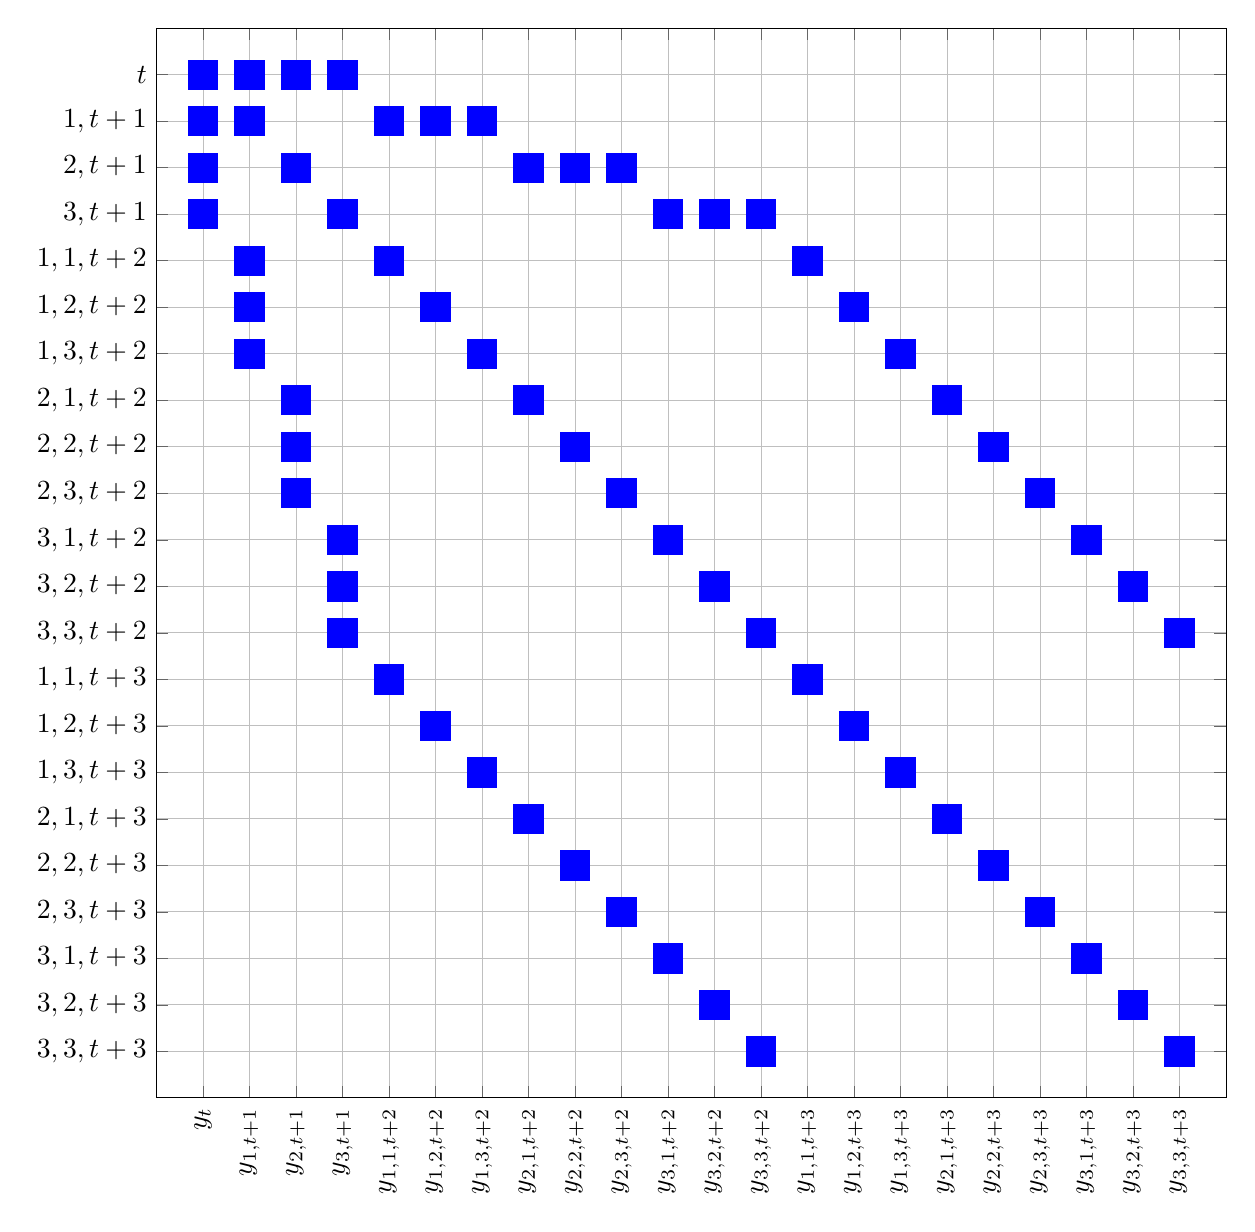
\begin{tikzpicture}

\begin{axis}[%
width=5.348in,
height=5.348in,
at={(1.854in,0.722in)},
scale only axis,
xmin=0,
xmax=23,
xtick={1,2,3,4,5,6,7,8,9,10,11,12,13,14,15,16,17,18,19,20,21,22},
xticklabels={{$y_t$},{$y_{1,t+1}$},{$y_{2,t+1}$},{$y_{3,t+1}$},{$y_{1,1,t+2}$},{$y_{1,2,t+2}$},{$y_{1,3,t+2}$},{$y_{2,1,t+2}$},{$y_{2,2,t+2}$},{$y_{2,3,t+2}$},{$y_{3,1,t+2}$},{$y_{3,2,t+2}$},{$y_{3,3,t+2}$},{$y_{1,1,t+3}$},{$y_{1,2,t+3}$},{$y_{1,3,t+3}$},{$y_{2,1,t+3}$},{$y_{2,2,t+3}$},{$y_{2,3,t+3}$},{$y_{3,1,t+3}$},{$y_{3,2,t+3}$},{$y_{3,3,t+3}$}},
xticklabel style={rotate=90},
y dir=reverse,
ymin=0,
ymax=23,
ytick={1,2,3,4,5,6,7,8,9,10,11,12,13,14,15,16,17,18,19,20,21,22},
yticklabels={$t$,{$1,t+1$},{$2,t+1$},{$3,t+1$},{$1,1,t+2$},{$1,2,t+2$},{$1,3,t+2$},{$2,1,t+2$},{$2,2,t+2$},{$2,3,t+2$},{$3,1,t+2$},{$3,2,t+2$},{$3,3,t+2$},{$1,1,t+3$},{$1,2,t+3$},{$1,3,t+3$},{$2,1,t+3$},{$2,2,t+3$},{$2,3,t+3$},{$3,1,t+3$},{$3,2,t+3$},{$3,3,t+3$}},
axis background/.style={fill=white},
xmajorgrids,
ymajorgrids
]
\addplot [color=blue, only marks, mark size=5.3pt, mark=square*, mark options={solid, blue}, forget plot]
  table[row sep=crcr]
   \end{center}

\end{frame}


\begin{frame}%[c]{}
   \frametitle{Stochastic perfect foresight models}
   \framesubtitle{order p}


   \[
      \scalebox{0.7}{$%
            \begin{split}
               \sum_{i_1=1}^m \omega_{i_1} & f\left({\color{blue}y_{t-1}}, {\color{red}y_t}, y_{t+1}^{i_1}, \varepsilon_t \right) = 0                                                                                                   \\
               \sum_{i_2=1}^m \omega_{i_2} & f\left({\color{red}y_{t}}, y_{t+1}^{i_1}, y_{t+1}^{i_2,i_1}, \epsilon_{i_1} \right) = 0\,\, \forall\, i_1\in \{1,\dots,m\}                                                                 \\
               \sum_{i_3=1}^m \omega_{i_3} & f\left(y_{t+1}^{i_1}, y_{t+2}^{i_2, i_1}, y_{t+3}^{i_3,i_2,i_1}, \epsilon_{i_2} \right) = 0\,\,  \forall\, (i_1,i_2)\in \{1,\dots,m\}^2                                                    \\
               \sum_{i_4=1}^m \omega_{i_4} & f\left(y_{t+2}^{i_2,i_1}, y_{t+3}^{i_3,i_2,i_1}, y_{t+3}^{i_4,\ldots,i_1}, \epsilon_{i_3} \right) = 0\,\,  \forall\, (i_1,i_2,i_3)\in \{1,\dots,m\}^3                                      \\
                                           & \vdots                                                                                                                                                                                     \\
               \sum_{i_p=1}^m \omega_{i_p} & f\left(y_{t+p-2}^{i_{p-2},\ldots,i_1}, y_{t+p-1}^{i_{p-1},\ldots,i_1}, y_{t+p}^{i_p,\ldots,i_1}, \epsilon_{i_{p-1}} \right) = 0\,\,  \forall\, (i_1,\ldots,i_{p-1})\in \{1,\dots,m\}^{p-1} \\
                                           & f\left(y_{t+p-1}^{i_{p-1},\ldots,i_1}, y_{t+p}^{i_{p},\ldots,i_1}, y_{t+p+1}^{i_p,\ldots,i_1}, \epsilon_{i_{p}} \right) = 0\,\,  \forall\, (i_1,\ldots,i_{p})\in \{1,\dots,m\}^{p}         \\
                                           & f\left(y_{t+p}^{i_{p},\ldots,i_1}, y_{t+p+1}^{i_{p},\ldots,i_1}, y_{t+p+2}^{i_p,\ldots,i_1}, 0 \right) = 0\,\,  \forall\, (i_1,\ldots,i_{p})\in \{1,\dots,m\}^{p}                          \\
                                           & \vdots                                                                                                                                                                                     \\
                                           & f\left(y_{t+H-2}^{i_{p},\ldots,i_1}, y_{t+H-1}^{i_{p},\ldots,i_1}, {\color{blue}y^{\star}}, 0 \right) = 0\,\,  \forall\, (i_1,\ldots,i_{p})\in \{1,\dots,m\}^{p}
            \end{split}$%
      }
   \]

\end{frame}


\begin{frame}%[c]{}
   \frametitle{Stochastic perfect foresight models}
   \framesubtitle{order p}

   \begin{itemize}

      \item Perfect $m$-ary tree of height $p$.\newline

      \item The root, at height 0, is $\sum_{i_1=1}^m \omega_{i_1}f\left(y_{t-1}, y_t, y_{t+1}^{i_1}, \varepsilon_t \right)$.\newline

      \item All the nodes from height 1 to $p-1$ are approximate integrals.\newline

      \item The $m^p$ terminal nodes at height $p$ are deterministic problems.\newline

      \item The $m^p$ leafs are deterministic paths to the steady state.\newline

      \item The size of the tree increases exponentially with the approximation order ($p$) and polynomially with the number of quadrature points ($m$).

   \end{itemize}

\end{frame}


\begin{frame}%[c]{}
   \frametitle{Stochastic perfect foresight models}
   \framesubtitle{order p}

   \begin{itemize}

      \item The number of unknown vectors is:
            \[
               \begin{split}
                  \mathcal C(m,p,H) & = 1+m+m^2+\ldots+m^{p-1} + m^p(H-p) \\
                                    & = \frac{m^p-1}{m-1} + m^p(H-p)
               \end{split}
            \]

      \item[$\Rightarrow$] The jacobian square matrix has $n\mathcal C(m,p,H)$ columns.\newline

      \item Number of non zero $n\times n$ blocks is:
            \[
               \mathrm{nnz}(m,p,H) = 1+m+(2+m)\frac{m^p-m}{m-1}+3m^p(H-p)-m^p
            \]

      \item The size of the Jacobian increases exponentially with the order
            of the SEP, while the sparsity improves (the proportion of non-zero blocks tends to zero as either $m$ or $p$ approaches infinity).

   \end{itemize}

\end{frame}


\begin{frame}
   \frametitle{Stochastic perfect foresight models}
   \framesubtitle{Stacked jacobian sparsity (3 quadrature nodes)}
   \begin{center}
      \scalebox{.5}{
         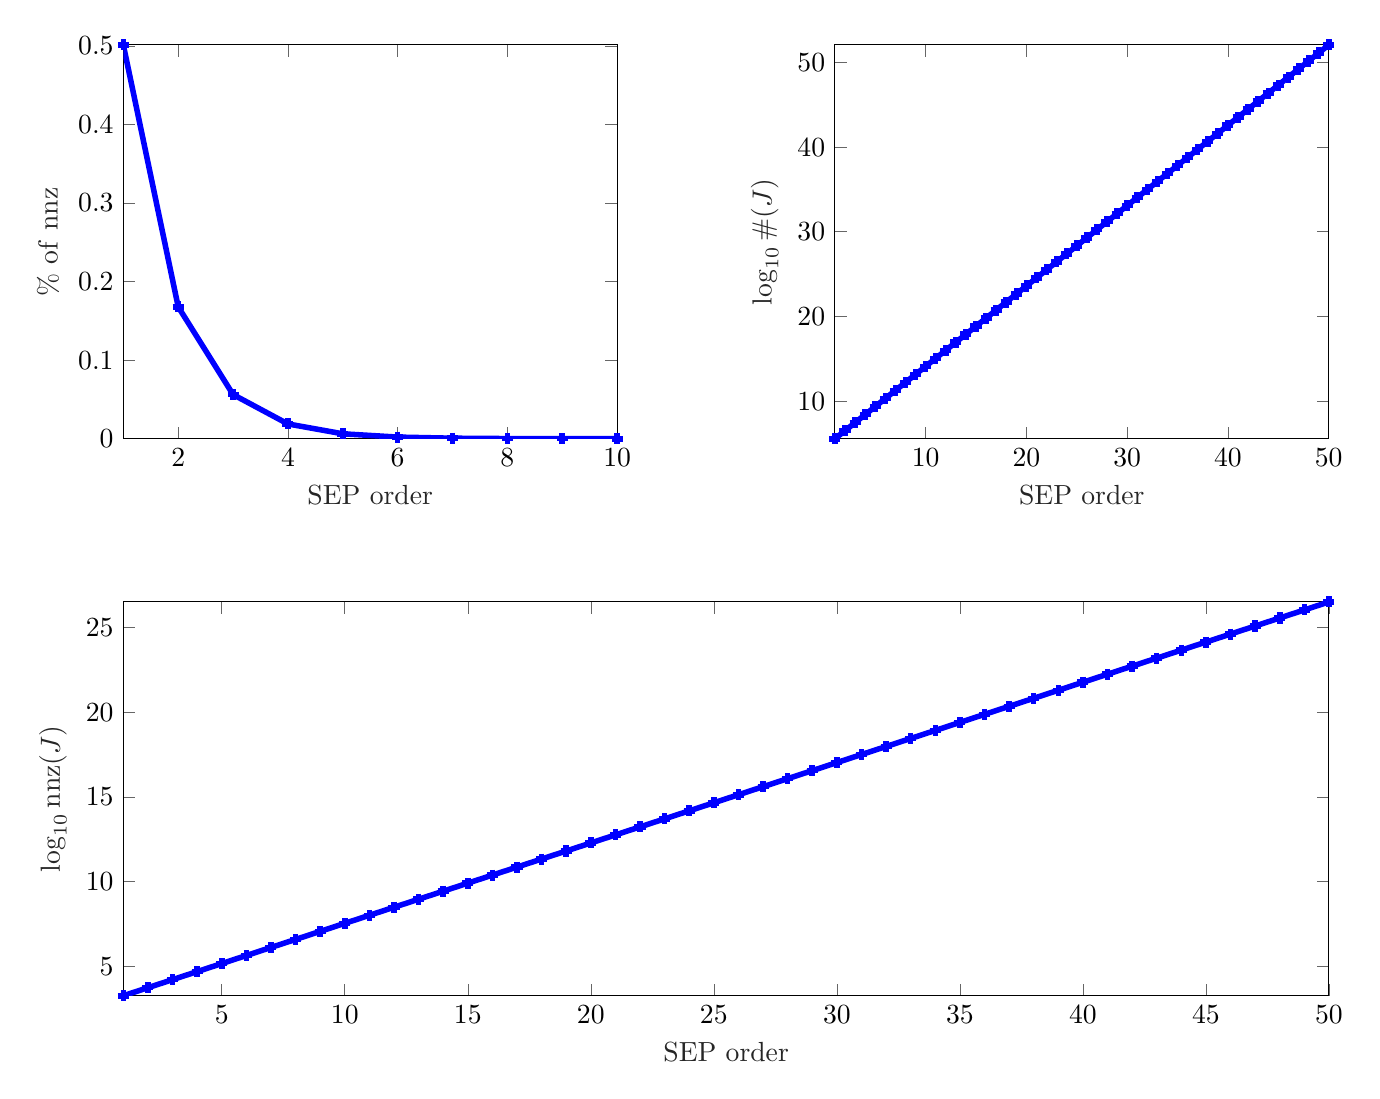
\begin{tikzpicture}

\begin{axis}[%
width=2.469in,
height=1.969in,
at={(1.011in,3.427in)},
scale only axis,
xmin=1,
xmax=10,
xlabel style={font=\color{white!15!black}},
xlabel={SEP order},
ymin=2.66694292244316e-05,
ymax=0.501112962942249,
ylabel style={font=\color{white!15!black}},
ylabel={\% of \textrm{nnz}},
axis background/.style={fill=white}
]
\addplot [color=blue, line width=2.0pt, mark=+, mark options={solid, blue}, forget plot]
  table[row sep=crcr]{%
1	0.501112962942249\\
2	0.167910424365696\\
3	0.0562570312495603\\
4	0.0188481675061982\\
5	0.00631490317024109\\
6	0.00211579511575775\\
7	0.000708910373247429\\
8	0.000237531070383557\\
9	7.95904874864273e-05\\
10	2.66694292244316e-05\\
};
\end{axis}

\begin{axis}[%
width=2.469in,
height=1.969in,
at={(4.569in,3.427in)},
scale only axis,
xmin=1,
xmax=50,
xlabel style={font=\color{white!15!black}},
xlabel={SEP order},
ymin=5.55340236797682,
ymax=52.067198471826,
ylabel style={font=\color{white!15!black}},
ylabel={$\log_{10} \#(J)$},
axis background/.style={fill=white}
]
\addplot [color=blue, line width=2.0pt, mark=+, mark options={solid, blue}, forget plot]
  table[row sep=crcr]{%
1	5.55340236797682\\
2	6.50376290910506\\
3	7.45378028148364\\
4	8.4036678609487\\
5	9.35349692882154\\
6	10.3032912050233\\
7	11.2530584785312\\
8	12.2028011993421\\
9	13.1525200263442\\
10	14.1022150158086\\
11	15.0518860195035\\
12	16.0015328180202\\
13	16.9511551653859\\
14	17.9007528039531\\
15	18.8503254693288\\
16	19.7998728919647\\
17	20.7493947976264\\
18	21.6988909074867\\
19	22.6483609380894\\
20	23.5978046012692\\
21	24.5472216040543\\
22	25.4966116485615\\
23	26.4459744318867\\
24	27.3953096459915\\
25	28.3446169775868\\
26	29.2938961080128\\
27	30.2431467131156\\
28	31.1923684631197\\
29	32.141561022498\\
30	33.0907240498368\\
31	34.0398571976973\\
32	34.9889601124731\\
33	35.9380324342434\\
34	36.8870737966217\\
35	37.8360838265998\\
36	38.7850621443877\\
37	39.7340083632476\\
38	40.6829220893241\\
39	41.6318029214679\\
40	42.5806504510548\\
41	43.5294642617987\\
42	44.4782439295592\\
43	45.4269890221422\\
44	46.3756990990952\\
45	47.3243737114953\\
46	48.2730124017307\\
47	49.2216147032747\\
48	50.1701801404532\\
49	51.1187082282036\\
50	52.067198471826\\
};
\end{axis}

\begin{axis}[%
width=6.028in,
height=1.969in,
at={(1.011in,0.642in)},
scale only axis,
xmin=1,
xmax=50,
xlabel style={font=\color{white!15!black}},
xlabel={SEP order},
ymin=3.25333800532611,
ymax=26.5107204906326,
ylabel style={font=\color{white!15!black}},
ylabel={$\log_{10} \mathrm{nnz}(J)$},
axis background/.style={fill=white}
]
\addplot [color=blue, line width=2.0pt, mark=+, mark options={solid, blue}, forget plot]
  table[row sep=crcr]{%
1	3.25333800532611\\
2	3.72884056833997\\
3	4.20395709168124\\
4	4.6789369937063\\
5	5.15386362449636\\
6	5.62876481526546\\
7	6.10364980981508\\
8	6.57852162514956\\
9	7.05338119107904\\
10	7.52822873688531\\
11	8.0030642558466\\
12	8.47788766083959\\
13	8.95269883644407\\
14	9.42749765637164\\
15	9.90228398927531\\
16	10.3770577006655\\
17	10.8518186535207\\
18	11.3265667084589\\
19	11.801301723763\\
20	12.2760235553538\\
21	12.7507320567466\\
22	13.2254270790004\\
23	13.700108470663\\
24	14.1747760777154\\
25	14.6494297435131\\
26	15.1240693087261\\
27	15.5986946112774\\
28	16.0733054862795\\
29	16.5479017659687\\
30	17.0224832796381\\
31	17.4970498535683\\
32	17.9716013109562\\
33	18.4461374718414\\
34	18.9206581530305\\
35	19.3951631680196\\
36	19.8696523269135\\
37	20.3441254363435\\
38	20.8185822993817\\
39	21.2930227154536\\
40	21.7674464802471\\
41	22.241853385619\\
42	22.7162432194993\\
43	23.1906157657908\\
44	23.6649708042673\\
45	24.1393081104673\\
46	24.613627455585\\
47	25.087928606357\\
48	25.5622113249463\\
49	26.0364753688214\\
50	26.5107204906326\\
};
\end{axis}
\end{tikzpicture}%}
   \end{center}

\end{frame}


\begin{frame}
   \frametitle{Stochastic perfect foresight models}
   \framesubtitle{Stacked jacobian sparsity (11 quadrature nodes)}
   \begin{center}
      \scalebox{.5}{
         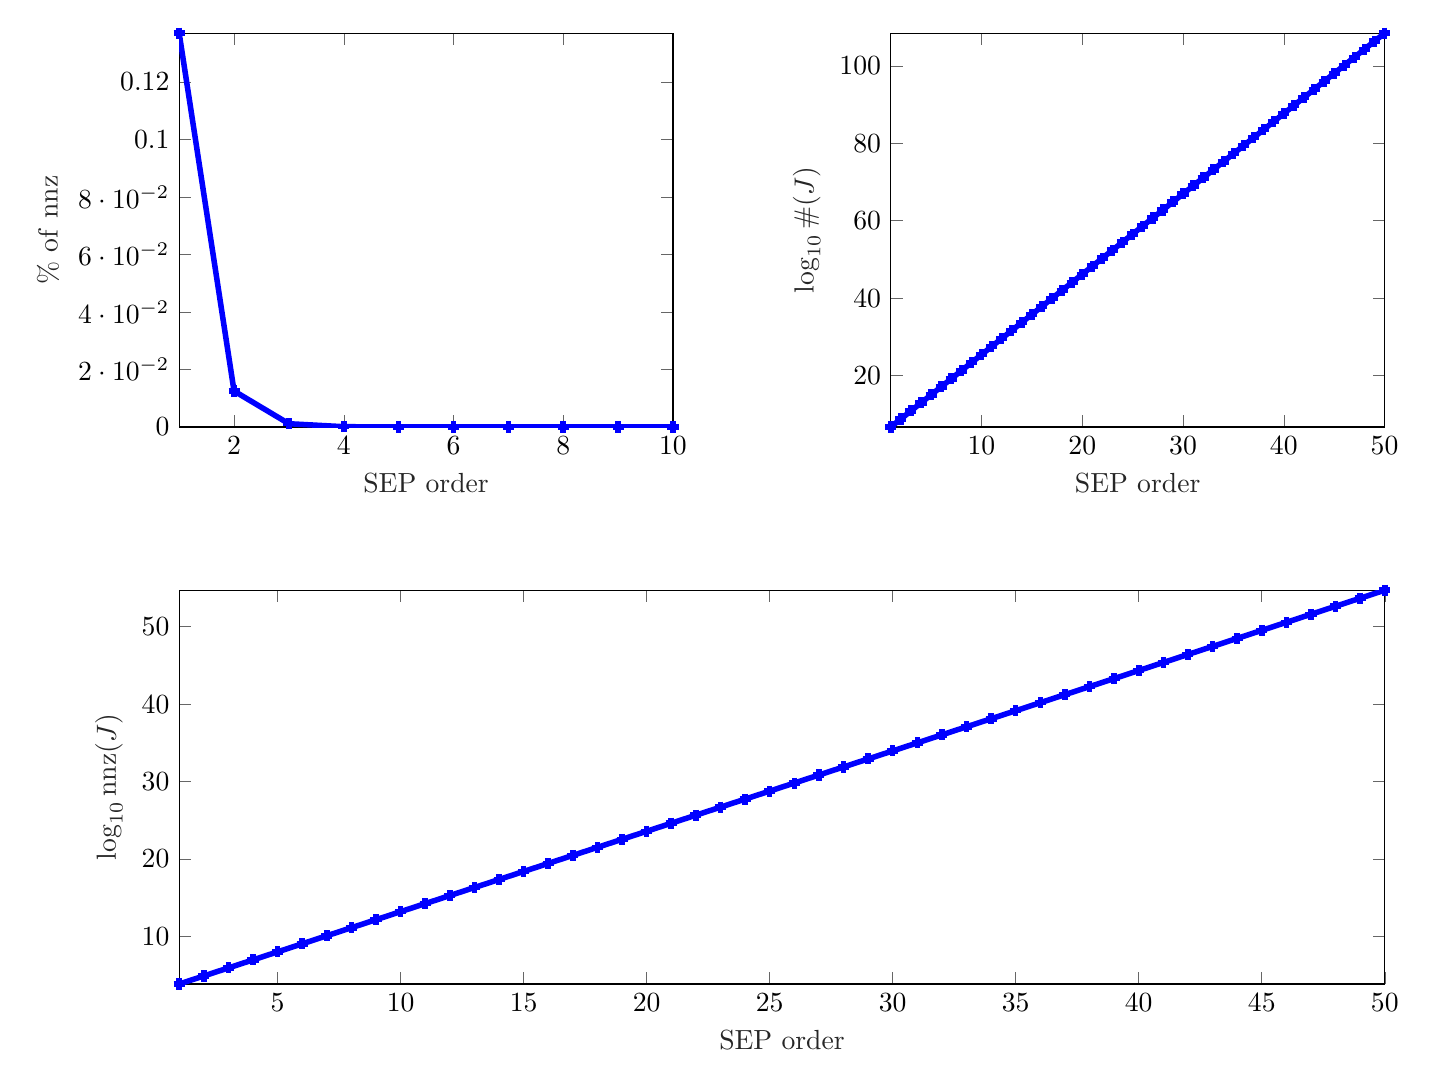
\begin{tikzpicture}

\begin{axis}[%
width=2.469in,
height=1.969in,
at={(1.011in,3.427in)},
scale only axis,
xmin=1,
xmax=10,
xlabel style={font=\color{white!15!black}},
xlabel={SEP order},
ymin=6.084323347125e-11,
ymax=0.136944600821501,
ylabel style={font=\color{white!15!black}},
ylabel={\% of \textrm{nnz}},
axis background/.style={fill=white}
]
\addplot [color=blue, line width=2.0pt, mark=+, mark options={solid, blue}, forget plot]
  table[row sep=crcr]{%
1	0.136944600821501\\
2	0.0125152964637865\\
3	0.00114355126031317\\
4	0.000104489544195705\\
5	9.54773929053422e-06\\
6	8.72448113019395e-07\\
7	7.97242027167421e-08\\
8	7.28538334518449e-09\\
9	6.65773341243252e-10\\
10	6.084323347125e-11\\
};
\end{axis}

\begin{axis}[%
width=2.469in,
height=1.969in,
at={(4.569in,3.427in)},
scale only axis,
xmin=1,
xmax=50,
xlabel style={font=\color{white!15!black}},
xlabel={SEP order},
ymin=6.68088822968024,
ymax=108.492029900309,
ylabel style={font=\color{white!15!black}},
ylabel={$\log_{10} \#(J)$},
axis background/.style={fill=white}
]
\addplot [color=blue, line width=2.0pt, mark=+, mark options={solid, blue}, forget plot]
  table[row sep=crcr]{%
1	6.68088822968024\\
2	8.75933606806731\\
3	10.8377290284155\\
4	12.9160966383485\\
5	14.9944413876069\\
6	17.0727632924228\\
7	19.1510621397509\\
8	21.2293376922529\\
9	23.3075897069579\\
10	25.3858179368954\\
11	27.464022131171\\
12	29.5422020348982\\
13	31.6203573891139\\
14	33.6984879306918\\
15	35.7765933922526\\
16	37.8546735020712\\
17	39.932727983983\\
18	42.0107565572859\\
19	44.0887589366407\\
20	46.1667348319681\\
21	48.2446839483435\\
22	50.3226059858884\\
23	52.4005006396585\\
24	54.4783675995294\\
25	56.5562065500781\\
26	58.6340171704624\\
27	60.7117991342949\\
28	62.7895521095157\\
29	64.8672757582593\\
30	66.9449697367186\\
31	69.0226336950054\\
32	71.1002672770053\\
33	73.1778701202296\\
34	75.2554418556621\\
35	77.3329821076013\\
36	79.4104904934984\\
37	81.4879666237892\\
38	83.5654101017221\\
39	85.64282052318\\
40	87.7201974764966\\
41	89.7975405422676\\
42	91.8748492931553\\
43	93.9521232936873\\
44	96.0293621000486\\
45	98.1065652598675\\
46	100.183732311994\\
47	102.26086278627\\
48	104.337956203296\\
49	106.415012074184\\
50	108.492029900309\\
};
\end{axis}

\begin{axis}[%
width=6.028in,
height=1.969in,
at={(1.011in,0.642in)},
scale only axis,
xmin=1,
xmax=50,
xlabel style={font=\color{white!15!black}},
xlabel={SEP order},
ymin=3.81743314411138,
ymax=54.7231362048742,
ylabel style={font=\color{white!15!black}},
ylabel={$\log_{10} \mathrm{nnz}(J)$},
axis background/.style={fill=white}
]
\addplot [color=blue, line width=2.0pt, mark=+, mark options={solid, blue}, forget plot]
  table[row sep=crcr]{%
1	3.81743314411138\\
2	4.85677720975119\\
3	5.89598466528318\\
4	6.93516947305116\\
5	7.97434193930862\\
6	9.01350290008908\\
7	10.0526523245181\\
8	11.0917901008391\\
9	12.130916108198\\
10	13.1700302231673\\
11	14.2091323203052\\
12	15.2482222721687\\
13	16.2872999492766\\
14	17.3263652200656\\
15	18.3654179508459\\
16	19.4044580057553\\
17	20.4434852467112\\
18	21.4824995333626\\
19	22.52150072304\\
20	23.5604886707037\\
21	24.5994632288914\\
22	25.6384242476639\\
23	26.6773715745489\\
24	27.7163050544843\\
25	28.7552245297587\\
26	29.7941298399508\\
27	30.8330208218671\\
28	31.8718973094775\\
29	32.9107591338493\\
30	33.949606123079\\
31	34.9884381022224\\
32	36.0272548932223\\
33	37.0660563148345\\
34	38.1048421825507\\
35	39.1436123085203\\
36	40.1823665014689\\
37	41.2211045666143\\
38	42.2598263055807\\
39	43.2985315163097\\
40	44.337219992968\\
41	45.3758915258535\\
42	46.4145459012973\\
43	47.4531829015633\\
44	48.491802304744\\
45	49.5304038846534\\
46	50.5689874107164\\
47	51.6075526478545\\
48	52.6460993563675\\
49	53.6846272918117\\
50	54.7231362048742\\
};
\end{axis}
\end{tikzpicture}%}
   \end{center}

\end{frame}


\begin{frame}
   \frametitle{Stochastic perfect foresight models}
   \framesubtitle{Stacked jacobian sparsity (order 2)}
   \begin{center}
      \scalebox{.5}{
         % This file was created by matlab2tikz.
%
%The latest updates can be retrieved from
%  http://www.mathworks.com/matlabcentral/fileexchange/22022-matlab2tikz-matlab2tikz
%where you can also make suggestions and rate matlab2tikz.
%
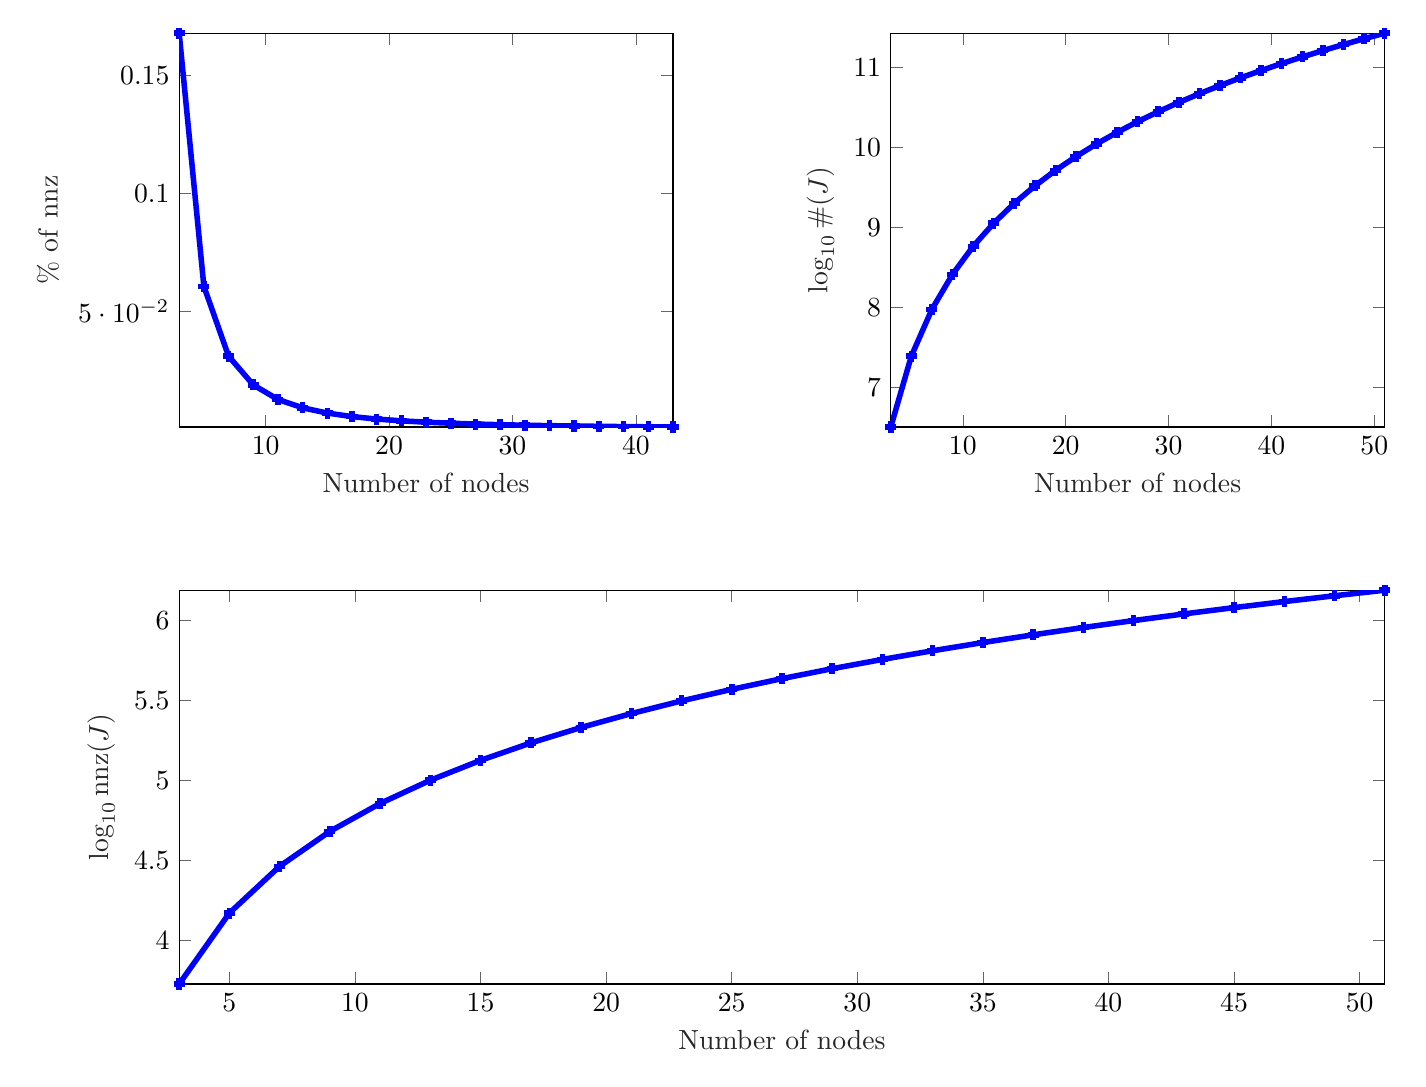
\begin{tikzpicture}

\begin{axis}[%
width=2.469in,
height=1.969in,
at={(1.011in,3.427in)},
scale only axis,
xmin=3,
xmax=43,
xlabel style={font=\color{white!15!black}},
xlabel={Number of nodes},
ymin=0.000819343796654361,
ymax=0.167910424365696,
ylabel style={font=\color{white!15!black}},
ylabel={\% of \textrm{nnz}},
axis background/.style={fill=white}
]
\addplot [color=blue, line width=2.0pt, mark=+, mark options={solid, blue}, forget plot]
  table[row sep=crcr]{%
3	0.167910424365696\\
5	0.0605245449707222\\
7	0.0308938622737026\\
9	0.0186931416617545\\
11	0.0125152964637865\\
13	0.00896146569394665\\
15	0.00673148840537474\\
17	0.00524102910447069\\
19	0.0041958824403334\\
21	0.00343482608310586\\
23	0.00286350620414749\\
25	0.00242372014104406\\
27	0.00207798444739654\\
29	0.0018012753028856\\
31	0.0015763698653937\\
33	0.00139110005099371\\
35	0.00123667143013247\\
37	0.00110660000835429\\
39	0.000996020345370709\\
41	0.000901223862000988\\
43	0.000819343796654361\\
};
\end{axis}

\begin{axis}[%
width=2.469in,
height=1.969in,
at={(4.569in,3.427in)},
scale only axis,
xmin=3,
xmax=51,
xlabel style={font=\color{white!15!black}},
xlabel={Number of nodes},
ymin=6.50376290910506,
ymax=11.4236987830146,
ylabel style={font=\color{white!15!black}},
ylabel={$\log_{10} \#(J)$},
axis background/.style={fill=white}
]
\addplot [color=blue, line width=2.0pt, mark=+, mark options={solid, blue}, forget plot]
  table[row sep=crcr]{%
3	6.50376290910506\\
5	7.39026259540805\\
7	7.97443845981601\\
9	8.41084183135269\\
11	8.75933606806731\\
13	9.04946711837303\\
15	9.29800731188404\\
17	9.51539925017548\\
19	9.70858778706756\\
21	9.88242637517064\\
23	10.0404407254452\\
25	10.1852728874617\\
27	10.3189539129485\\
29	10.4430788436229\\
31	10.5589232185153\\
33	10.6675230912579\\
35	10.7697314669425\\
37	10.866259035161\\
39	10.9577041675152\\
41	11.0445754055698\\
43	11.1273085880072\\
45	11.2062800809681\\
47	11.2818171293633\\
49	11.3542060497057\\
51	11.4236987830146\\
};
\end{axis}

\begin{axis}[%
width=6.028in,
height=1.969in,
at={(1.011in,0.642in)},
scale only axis,
xmin=3,
xmax=51,
xlabel style={font=\color{white!15!black}},
xlabel={Number of nodes},
ymin=3.72884056833997,
ymax=6.18897008408768,
ylabel style={font=\color{white!15!black}},
ylabel={$\log_{10} \mathrm{nnz}(J)$},
axis background/.style={fill=white}
]
\addplot [color=blue, line width=2.0pt, mark=+, mark options={solid, blue}, forget plot]
  table[row sep=crcr]{%
3	3.72884056833997\\
5	4.17219412846693\\
7	4.46431066592589\\
9	4.68252412854228\\
11	4.85677720975119\\
13	5.00184616494759\\
15	5.1261184139642\\
17	5.23481582160788\\
19	5.33141109875549\\
21	5.41833112732033\\
23	5.49733885384933\\
25	5.56975535930212\\
27	5.63659620571961\\
29	5.69865893811197\\
31	5.7565813426166\\
33	5.81088145779331\\
35	5.86198579467581\\
37	5.91024970431781\\
39	5.95597237721597\\
41	5.99940808773183\\
43	6.04077475797337\\
45	6.08026057317681\\
47	6.11802915751285\\
49	6.15422367061031\\
51	6.18897008408768\\
};
\end{axis}
\end{tikzpicture}%}
   \end{center}

\end{frame}


\begin{frame}
   \frametitle{Stochastic perfect foresight models}
   \framesubtitle{Stacked jacobian sparsity (order 10)}
   \begin{center}
      \scalebox{.5}{
         % This file was created by matlab2tikz.
%
%The latest updates can be retrieved from
%  http://www.mathworks.com/matlabcentral/fileexchange/22022-matlab2tikz-matlab2tikz
%where you can also make suggestions and rate matlab2tikz.
%
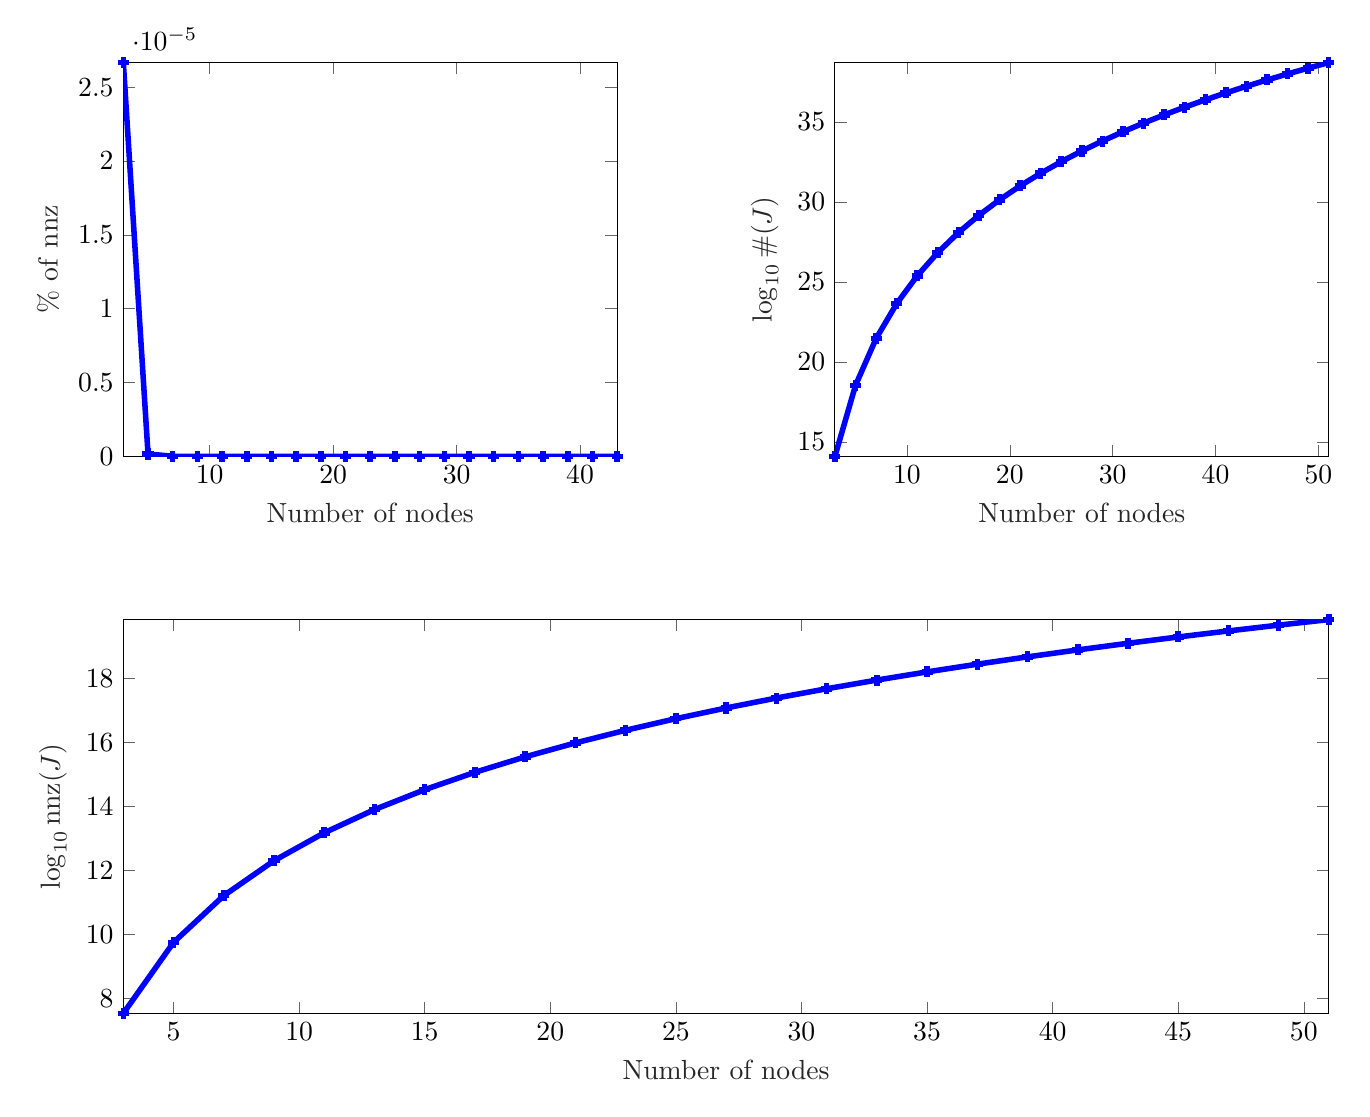
\begin{tikzpicture}

\begin{axis}[%
width=2.469in,
height=1.969in,
at={(1.011in,3.427in)},
scale only axis,
xmin=3,
xmax=43,
xlabel style={font=\color{white!15!black}},
xlabel={Number of nodes},
ymin=7.30514227228012e-17,
ymax=2.66694292244316e-05,
ylabel style={font=\color{white!15!black}},
ylabel={\% of \textrm{nnz}},
axis background/.style={fill=white}
]
\addplot [color=blue, line width=2.0pt, mark=+, mark options={solid, blue}, forget plot]
  table[row sep=crcr]{%
3	2.66694292244316e-05\\
5	1.61471747664182e-07\\
7	5.58478502567508e-09\\
9	4.52539959099029e-10\\
11	6.084323347125e-11\\
13	1.14483709351624e-11\\
15	2.73710731478755e-12\\
17	7.82952839432584e-13\\
19	2.57456983253181e-13\\
21	9.46368842400786e-14\\
23	3.81053019893826e-14\\
25	1.65528331506249e-14\\
27	7.66729383667823e-15\\
29	3.7523733956208e-15\\
31	1.92608092445839e-15\\
33	1.03075827693185e-15\\
35	5.72295046935379e-16\\
37	3.28312126737696e-16\\
39	1.93937340645338e-16\\
41	1.17617500604147e-16\\
43	7.30514227228012e-17\\
};
\end{axis}

\begin{axis}[%
width=2.469in,
height=1.969in,
at={(4.569in,3.427in)},
scale only axis,
xmin=3,
xmax=51,
xlabel style={font=\color{white!15!black}},
xlabel={Number of nodes},
ymin=14.1022150158086,
ymax=38.7090021494698,
ylabel style={font=\color{white!15!black}},
ylabel={$\log_{10} \#(J)$},
axis background/.style={fill=white}
]
\addplot [color=blue, line width=2.0pt, mark=+, mark options={solid, blue}, forget plot]
  table[row sep=crcr]{%
3	14.1022150158086\\
5	18.5380494174887\\
7	21.4602295883516\\
9	23.6429286429084\\
11	25.3858179368954\\
13	26.8367551245948\\
15	28.0796588588599\\
17	29.1667713025419\\
19	30.1328331572201\\
21	31.0021216425566\\
23	31.7922716938083\\
25	32.5164978344994\\
27	33.1849582950169\\
29	33.8056304131441\\
31	34.3848934492544\\
33	34.9279288477433\\
35	35.4390025350013\\
37	35.9216686606544\\
39	36.3789196372857\\
41	36.8132986168036\\
43	37.2269851524129\\
45	37.6218613694004\\
47	37.9995637358233\\
49	38.3615240372728\\
51	38.7090021494698\\
};
\end{axis}

\begin{axis}[%
width=6.028in,
height=1.969in,
at={(1.011in,0.642in)},
scale only axis,
xmin=3,
xmax=51,
xlabel style={font=\color{white!15!black}},
xlabel={Number of nodes},
ymin=7.52822873688531,
ymax=19.8316223294546,
ylabel style={font=\color{white!15!black}},
ylabel={$\log_{10} \mathrm{nnz}(J)$},
axis background/.style={fill=white}
]
\addplot [color=blue, line width=2.0pt, mark=+, mark options={solid, blue}, forget plot]
  table[row sep=crcr]{%
3	7.52822873688531\\
5	9.74614596330819\\
7	11.2072360488901\\
9	12.2985855761734\\
11	13.1700302231673\\
13	13.895498817017\\
15	14.5169506841496\\
17	15.0605069059906\\
19	15.5435378333297\\
21	15.978182075998\\
23	16.3732571016238\\
25	16.7353701719694\\
27	17.0696004022281\\
29	17.3799364612917\\
31	17.6695679793469\\
33	17.9410856785913\\
35	18.1966225222203\\
37	18.4379555850469\\
39	18.6665810733625\\
41	18.8837705631215\\
43	19.0906138309261\\
45	19.2880519394199\\
47	19.4769031226313\\
49	19.6578832733561\\
51	19.8316223294546\\
};
\end{axis}
\end{tikzpicture}%}
   \end{center}

\end{frame}


\begin{frame}
   \frametitle{Stochastic perfect foresight model}
   \framesubtitle{Sparse tree}

   \begin{itemize}

      \item Employing the complete $m$-ary tree presented above is
            infeasible for large values of $p$ or $m$.\newline

      \item Trimming the tree by eliminating branches with low
            probabilities (as determined by the products of quadrature
            weights) offers limited benefits, as the pruned tree would still
            expand exponentially with respect to $p$.\newline

      \item The trunk of the $m$-ary tree is defined by traversing the
            central nodes from one period to the next.\newline

      \item All branches that do not directly stem from the trunk are
            removed.\newline

      \item Fishbone tree $\Leftrightarrow$ Monomial rule, where
            innovations in different periods are treated as distinct
            shocks.

   \end{itemize}

\end{frame}


\begin{frame}[c]{}
   \frametitle{Tree of forward histories}
   \framesubtitle{Sparse tree}
   \begin{center}
      \begin{tikzpicture}[scale=.7]
         \tikzset{grow'=right,level distance=80pt}
         \tikzset{execute at begin node=\strut}
         \tikzset{every tree node/.style={anchor=base west}}
         \Tree [.$\varepsilon_t$
         [.$\epsilon_2$ ]
         [.$\epsilon_1$
         [.$\epsilon_2$ ]
         [.$\epsilon_1$
         [.$\epsilon_2$ ]
         [.$\epsilon_1$
         [.$\epsilon_2$ ]
         [.$\epsilon_1$ \edge[dashed]; {} \edge[dashed]; {} \edge[dashed]; {} ]
         [.$\epsilon_3$ ]
         ]
         [.$\epsilon_3$ ]
         ]
         [.$\epsilon_3$  ]
         ]
         [.$\epsilon_3$ ]
         ]
      \end{tikzpicture}

   \end{center}
\end{frame}


\begin{frame}
   \frametitle{Stochastic perfect foresight model}
   \framesubtitle{Sparse tree}

   \begin{itemize}

      \item The leaf on each terminal node is a deterministic path to the steady state.\newline

      \item The number of terminal nodes, $mp$, expands linearly with the SEP approximation order.\newline

      \item The number of unknown $n\times 1$ vectors to be solved for is:
            \[
               \begin{split}
                  \bar{\mathcal C}(m,p,H) & =  H+\sum_{i=1}^p(m-1)(H-i)                     \\
                                          & = \left( 1 + (m-1)p \right)H - \frac{p(p+1)}{2}
               \end{split}
            \]

   \end{itemize}

\end{frame}


\begin{frame}
   \frametitle{Stochastic perfect foresight model}
   \framesubtitle{Sparse tree}

   \begin{itemize}

      \item The number of non zero $n\times n$ blocks in the stacked Jacobian is:
            {\small
            \[
               \overline{\mathrm{nnz}}(m,p,H) = \underbrace{\overbrace{3H-2}^{\mathrm{EP}} + \overbrace{(m-1)p}^{\text{Approximate} \atop \text{integrals} }}_{\text{Along the trunk}} + (m-1)\sum_{i=1}^{p-1} \left( 3(H-1-i)+2  \right)
            \]}

            \medskip

      \item The Jacobian is smaller in size, with its growth occurring linearly in relation to \( p \) or \( m \); however, it is denser.

   \end{itemize}

\end{frame}


\begin{frame}
   \frametitle{Stochastic perfect foresight models}
   \framesubtitle{Stacked jacobian sparsity with sparse tree (3 quadrature nodes)}
   \begin{center}
      \scalebox{.5}{
         % This file was created by matlab2tikz.
%
%The latest updates can be retrieved from
%  http://www.mathworks.com/matlabcentral/fileexchange/22022-matlab2tikz-matlab2tikz
%where you can also make suggestions and rate matlab2tikz.
%
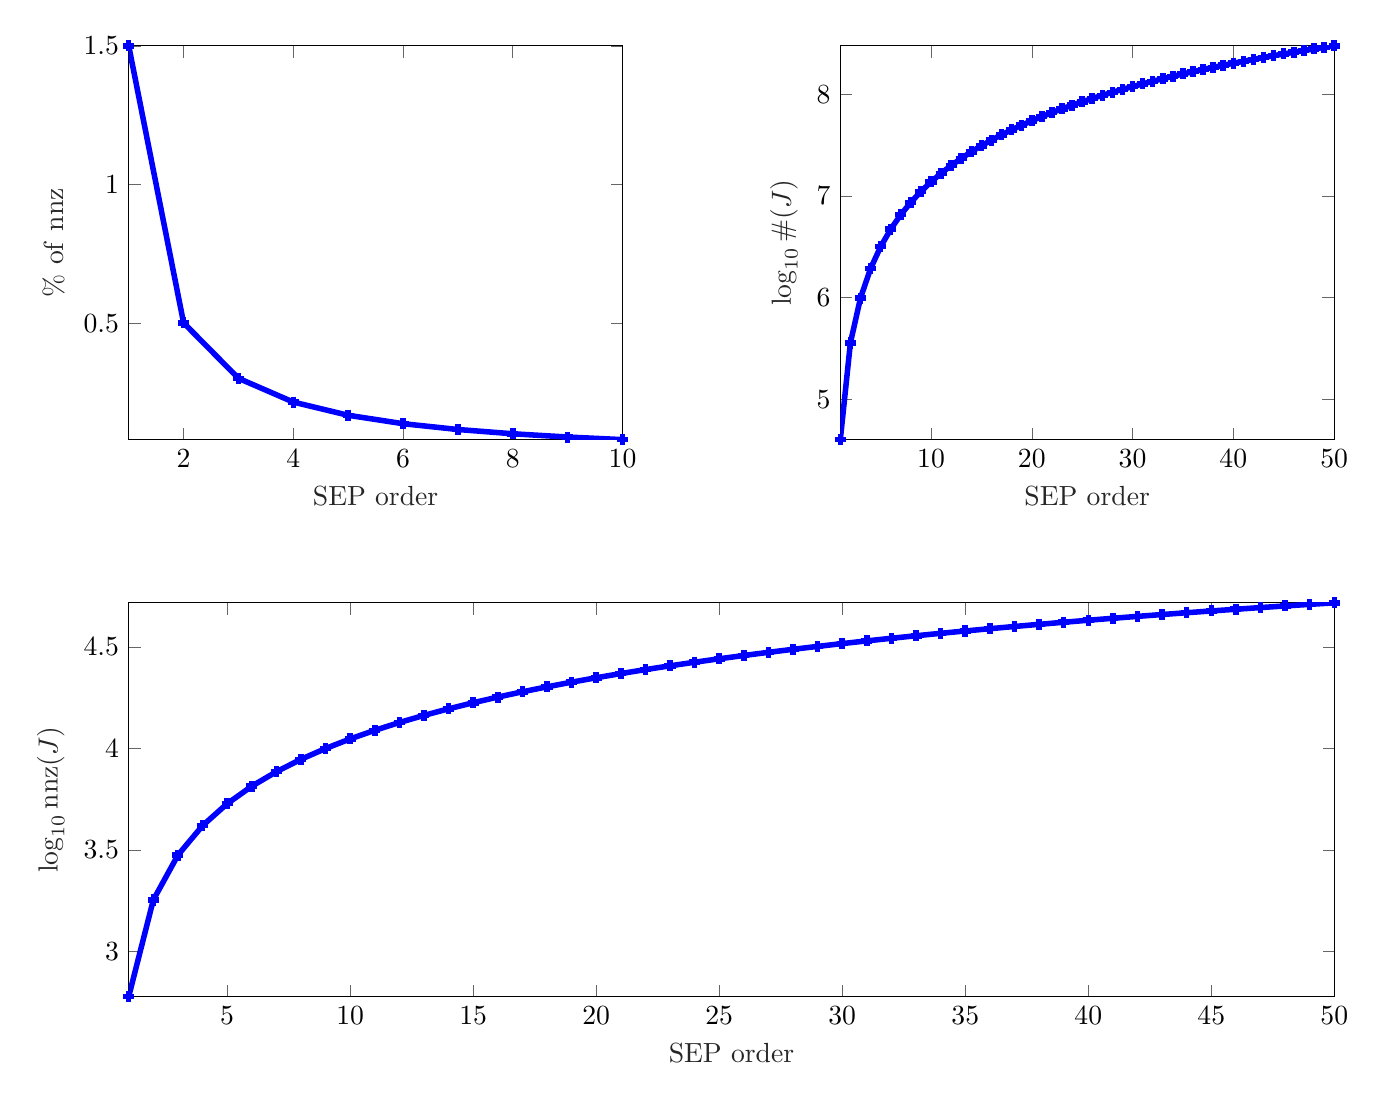
\begin{tikzpicture}

\begin{axis}[%
width=2.469in,
height=1.969in,
at={(1.011in,3.427in)},
scale only axis,
xmin=1,
xmax=10,
xlabel style={font=\color{white!15!black}},
xlabel={SEP order},
ymin=0.0808625336927224,
ymax=1.5,
ylabel style={font=\color{white!15!black}},
ylabel={\% of \textrm{nnz}},
axis background/.style={fill=white}
]
\addplot [color=blue, line width=2.0pt, mark=+, mark options={solid, blue}, forget plot]
  table[row sep=crcr]{%
1	1.5\\
2	0.501672240802676\\
3	0.301810865191147\\
4	0.216138328530259\\
5	0.168539325842697\\
6	0.138248847926267\\
7	0.117279124315872\\
8	0.101902173913043\\
9	0.0901442307692308\\
10	0.0808625336927224\\
};
\end{axis}

\begin{axis}[%
width=2.469in,
height=1.969in,
at={(4.569in,3.427in)},
scale only axis,
xmin=1,
xmax=50,
xlabel style={font=\color{white!15!black}},
xlabel={SEP order},
ymin=4.60205999132796,
ymax=8.47859895825379,
ylabel style={font=\color{white!15!black}},
ylabel={$\log_{10} \#(J)$},
axis background/.style={fill=white}
]
\addplot [color=blue, line width=2.0pt, mark=+, mark options={solid, blue}, forget plot]
  table[row sep=crcr]{%
1	4.60205999132796\\
2	5.55340236797682\\
3	5.99477276879463\\
4	6.28477893223767\\
5	6.50084000461779\\
6	6.67291946769706\\
7	6.81580108028527\\
8	6.93787561133092\\
9	7.04436663523737\\
10	7.13874781923009\\
11	7.22344661601468\\
12	7.30022632888714\\
13	7.37040826894203\\
14	7.4350081495284\\
15	7.49482361577285\\
16	7.55049251948047\\
17	7.60253294097924\\
18	7.65137141604352\\
19	7.6973633080479\\
20	7.74080781055805\\
21	7.78195919397938\\
22	7.82103537103453\\
23	7.85822451330932\\
24	7.89369022792125\\
25	7.92757565469111\\
26	7.96000674316749\\
27	7.99109489895027\\
28	8.02093913959278\\
29	8.04962786525862\\
30	8.0772403238994\\
31	8.10384783209221\\
32	8.12951479885936\\
33	8.15429958943394\\
34	8.17825525808856\\
35	8.20143017314616\\
36	8.22386855266536\\
37	8.24561092569489\\
38	8.26669453117249\\
39	8.28715366431799\\
40	8.30701997860167\\
41	8.32632274995404\\
42	8.34508910874473\\
43	8.36334424413653\\
44	8.38111158467034\\
45	8.39841295832332\\
46	8.41526873477792\\
47	8.43169795222291\\
48	8.44771843066126\\
49	8.46334687341229\\
50	8.47859895825379\\
};
\end{axis}

\begin{axis}[%
width=6.028in,
height=1.969in,
at={(1.011in,0.642in)},
scale only axis,
xmin=1,
xmax=50,
xlabel style={font=\color{white!15!black}},
xlabel={SEP order},
ymin=2.77815125038364,
ymax=4.71642073384656,
ylabel style={font=\color{white!15!black}},
ylabel={$\log_{10} \mathrm{nnz}(J)$},
axis background/.style={fill=white}
]
\addplot [color=blue, line width=2.0pt, mark=+, mark options={solid, blue}, forget plot]
  table[row sep=crcr]{%
1	2.77815125038364\\
2	3.25382243870807\\
3	3.47450763911698\\
4	3.6195107208385\\
5	3.72754125702856\\
6	3.81358098856819\\
7	3.8850217948623\\
8	3.94605906038512\\
9	3.99930457233835\\
10	4.04649516433471\\
11	4.088844562727\\
12	4.12723441916323\\
13	4.16232538919068\\
14	4.19462532948386\\
15	4.22453306260609\\
16	4.2523675144599\\
17	4.27838772520928\\
18	4.30280696274142\\
19	4.32580290874361\\
20	4.34752515999869\\
21	4.36810085170935\\
22	4.38763894023693\\
23	4.40623351137432\\
24	4.42396636868029\\
25	4.44090908206522\\
26	4.45712462630341\\
27	4.4726687041948\\
28	4.48759082451605\\
29	4.50193518734897\\
30	4.51574141666937\\
31	4.52904517076577\\
32	4.54187865414934\\
33	4.55427104943663\\
34	4.56624888376394\\
35	4.57783634129274\\
36	4.58905553105234\\
37	4.59992671756711\\
38	4.61046852030591\\
39	4.62069808687866\\
40	4.6306312440205\\
41	4.64028262969668\\
42	4.64966580909203\\
43	4.65879337678793\\
44	4.66767704705483\\
45	4.67632773388132\\
46	4.68475562210862\\
47	4.69297023083112\\
48	4.70098047005029\\
49	4.70879469142581\\
50	4.71642073384656\\
};
\end{axis}
\end{tikzpicture}%}
   \end{center}

\end{frame}


\begin{frame}
   \frametitle{Stochastic perfect foresight models}
   \framesubtitle{Stacked jacobian sparsity with sparse tree (11 quadrature nodes)}
   \begin{center}
      \scalebox{.5}{
         % This file was created by matlab2tikz.
%
%The latest updates can be retrieved from
%  http://www.mathworks.com/matlabcentral/fileexchange/22022-matlab2tikz-matlab2tikz
%where you can also make suggestions and rate matlab2tikz.
%
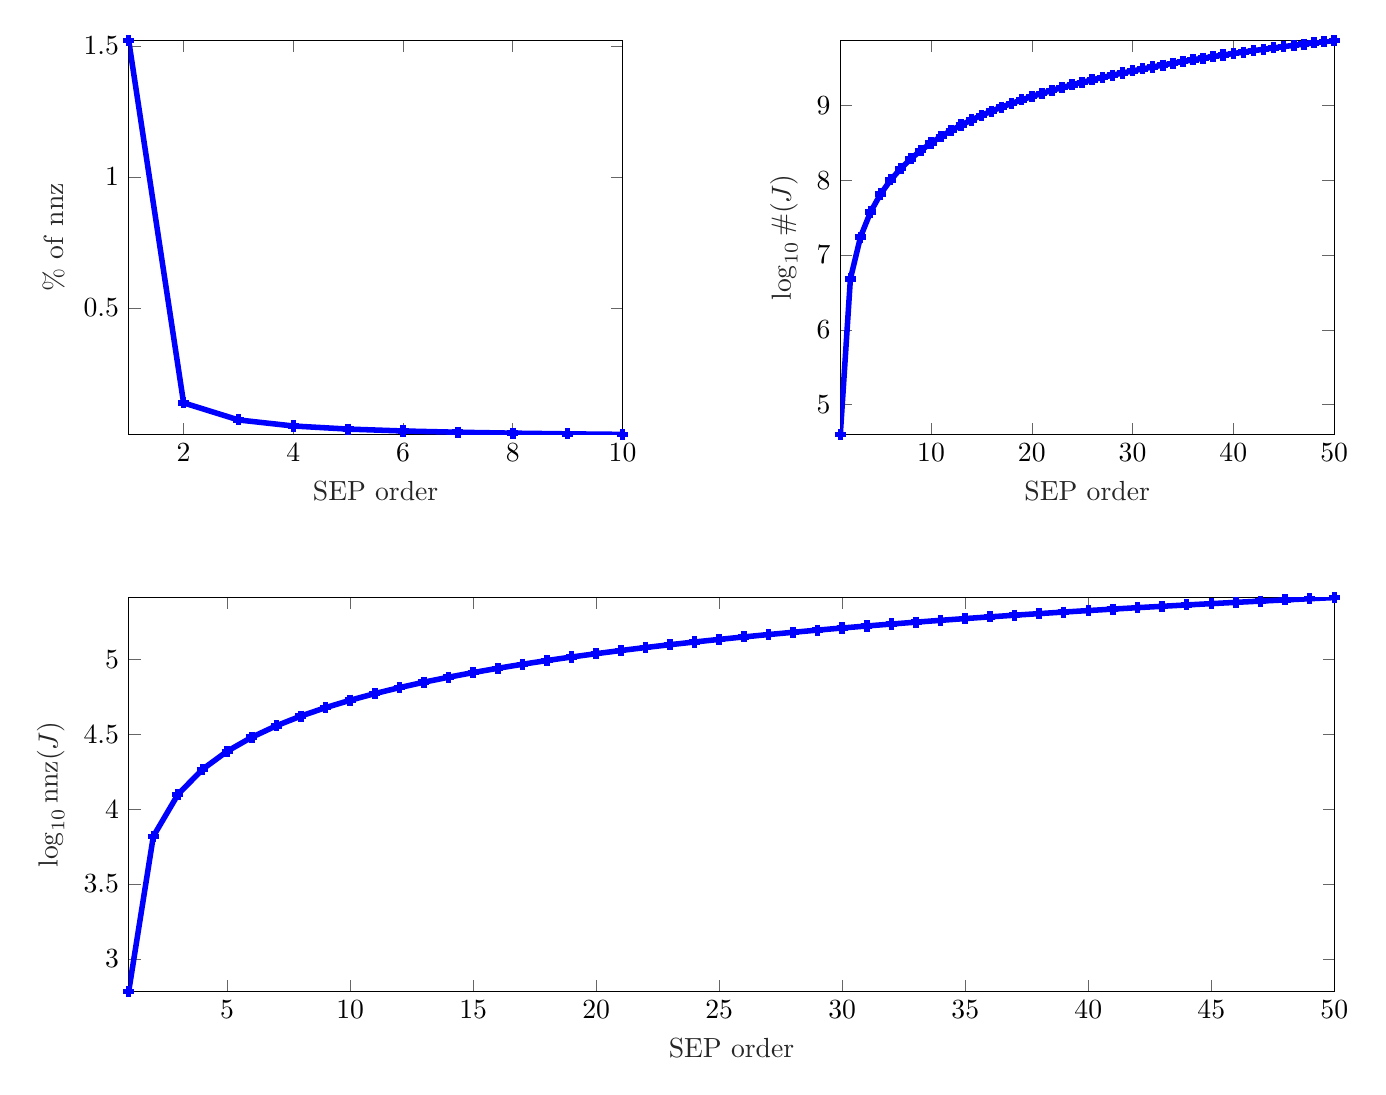
\begin{tikzpicture}

\begin{axis}[%
width=2.469in,
height=1.969in,
at={(1.011in,3.427in)},
scale only axis,
xmin=1,
xmax=10,
xlabel style={font=\color{white!15!black}},
xlabel={SEP order},
ymin=0.0169039476294386,
ymax=1.52,
ylabel style={font=\color{white!15!black}},
ylabel={\% of \textrm{nnz}},
axis background/.style={fill=white}
]
\addplot [color=blue, line width=2.0pt, mark=+, mark options={solid, blue}, forget plot]
  table[row sep=crcr]{%
1	1.52\\
2	0.137153103563312\\
3	0.0719884524035448\\
4	0.0488811552377214\\
5	0.0370492303002591\\
6	0.0298586668646816\\
7	0.0250264155353259\\
8	0.0215558528207161\\
9	0.0189425823895521\\
10	0.0169039476294386\\
};
\end{axis}

\begin{axis}[%
width=2.469in,
height=1.969in,
at={(4.569in,3.427in)},
scale only axis,
xmin=1,
xmax=50,
xlabel style={font=\color{white!15!black}},
xlabel={SEP order},
ymin=4.60205999132796,
ymax=9.86849176204614,
ylabel style={font=\color{white!15!black}},
ylabel={$\log_{10} \#(J)$},
axis background/.style={fill=white}
]
\addplot [color=blue, line width=2.0pt, mark=+, mark options={solid, blue}, forget plot]
  table[row sep=crcr]{%
1	4.60205999132796\\
2	6.68088822968024\\
3	7.24027210994752\\
4	7.57633674228234\\
5	7.8169700377573\\
6	8.00433212351301\\
7	8.1576383661977\\
8	8.28727847054909\\
9	8.39951035450695\\
10	8.49839671478223\\
11	8.58672510942289\\
12	8.66649139792393\\
13	8.73917378147269\\
14	8.80589765868881\\
15	8.86753966784973\\
16	8.92479599579791\\
17	8.97822873875784\\
18	9.02829826895088\\
19	9.07538638873478\\
20	9.11981325007222\\
21	9.16184995135124\\
22	9.20172807261968\\
23	9.23964700091456\\
24	9.27577963316158\\
25	9.31027686962276\\
26	9.34327119320426\\
27	9.37487954909179\\
28	9.40520568268085\\
29	9.43434205366462\\
30	9.462371415268\\
31	9.48936812655377\\
32	9.51539925017548\\
33	9.54052547634119\\
34	9.56480190499306\\
35	9.58827871153555\\
36	9.6110017163168\\
37	9.63301287409271\\
38	9.65435069659739\\
39	9.6750506188992\\
40	9.69514531828422\\
41	9.71466499286254\\
42	9.7336376058521\\
43	9.75208910049219\\
44	9.7700435897246\\
45	9.78752352411589\\
46	9.804549840949\\
47	9.82114209696252\\
48	9.83731858684365\\
49	9.85309644927124\\
50	9.86849176204614\\
};
\end{axis}

\begin{axis}[%
width=6.028in,
height=1.969in,
at={(1.011in,0.642in)},
scale only axis,
xmin=1,
xmax=50,
xlabel style={font=\color{white!15!black}},
xlabel={SEP order},
ymin=2.78390357927274,
ymax=5.41138060986319,
ylabel style={font=\color{white!15!black}},
ylabel={$\log_{10} \mathrm{nnz}(J)$},
axis background/.style={fill=white}
]
\addplot [color=blue, line width=2.0pt, mark=+, mark options={solid, blue}, forget plot]
  table[row sep=crcr]{%
1	2.78390357927274\\
2	3.81809386914664\\
3	4.09753494721728\\
4	4.26547820358064\\
5	4.38574922767528\\
6	4.47940253687398\\
7	4.55603701745574\\
8	4.62084368020266\\
9	4.67694953936863\\
10	4.7263848533295\\
11	4.7705427427666\\
12	4.81042071630634\\
13	4.84675759262467\\
14	4.8801158751896\\
15	4.91093374285252\\
16	4.93955918590741\\
17	4.96627317495952\\
18	4.99130583674195\\
19	5.0148480261775\\
20	5.03705978267814\\
21	5.05807662614571\\
22	5.07801432286479\\
23	5.09697254691112\\
24	5.11503773067138\\
25	5.13228531086859\\
26	5.14878151768452\\
27	5.16458481416811\\
28	5.17974706488186\\
29	5.19431449269512\\
30	5.20832846820221\\
31	5.22182616571611\\
32	5.23484111201639\\
33	5.2474036482265\\
34	5.259541320818\\
35	5.27127921440412\\
36	5.28264023642194\\
37	5.29364536181574\\
38	5.30431384428127\\
39	5.31466339940944\\
40	5.32471036409878\\
41	5.33446983583388\\
42	5.34395579480613\\
43	5.3531812113523\\
44	5.36215814077947\\
45	5.3708978073127\\
46	5.37941067862911\\
47	5.38770653221734\\
48	5.39579451461515\\
49	5.40368319442316\\
50	5.41138060986319\\
};
\end{axis}
\end{tikzpicture}%}
   \end{center}

\end{frame}


\begin{frame}
   \frametitle{Stochastic perfect foresight model}
   \framesubtitle{Sparse tree, equations for SEP($p$)}

   \begin{itemize}

      \item Let $y_{t,s}^i$ represent the vector of endogenous variables
            at time $s>t$ along a branch that diverges from the trunk at
            time $t$ due to the anticipated shock (integration
            node) $\epsilon_i$.\newline

      \item The sequence $y_t$ (the
            root), $y_{t,t+1}^1$, $y_{t+1,t+2}^1$,
            \dots, $y_{t+p-1,t+p}^1$ represents the path of the
            endogenous variables along the trunk.\newline

      \item Approximate integrals are located along the trunk.\newline

      \item In period $t$ we have:
            \[
               \sum_{i=1}^m\omega_i f\left( y_{t-1}, y_t, y_{t, t+1}^i, \varepsilon_t \right) = 0
            \]

   \end{itemize}

\end{frame}


\begin{frame}
   \frametitle{Stochastic perfect foresight model}
   \framesubtitle{Sparse tree, equations for SEP($p$)}

   \begin{itemize}

      \item In period $t+1$ we have:
            \[
               \begin{split}
                   & \sum_{i=1}^m\omega_i f\left( y_t, y_{t,t+1}^1, y_{t+1, t+2}^i, \epsilon_i \right) = 0 \\
                   & f\left(y_t, y_{t,t+1}^i, y_{t,t+2}^i, 0\right) = 0\quad \forall\, i\in\{2,\ldots,m\}
               \end{split}
            \]

            \medskip

      \item In period $t+2$ we have:
            \[
               \begin{split}
                   & \sum_{i=1}^m\omega_i f\left( y_{t,t+1}^1, y_{t+1,t+1}^1, y_{t+2, t+3}^i, \epsilon_i \right) = 0   \\
                   & f\left(y_{t,t+1}^i, y_{t,t+2}^i, y_{t,t+3}^i, 0\right) = 0\quad \forall\, i\in\{2,\ldots,m\}      \\
                   & f\left(y_{t,t+1}^1, y_{t+1,t+2}^i, y_{t+1, t+3}^i, 0\right) = 0\quad \forall\, i\in\{2,\ldots,m\} \\
               \end{split}
            \]

   \end{itemize}

\end{frame}


\begin{frame}
   \frametitle{Stochastic perfect foresight model}
   \framesubtitle{Sparse tree, equations for SEP($p$)}

   \begin{itemize}

      \item In period $t+h$, with $h<p$, we have:
            \[
               \begin{split}
                   & \sum_{i=1}^m\omega_i f\left( y_{t+h-2,t+h-1}^1, y_{t+h-1,t+h}^1, y_{t+h, t+h+1}^i, \epsilon_i \right) = 0      \\
                   & f\left(y_{t,t+h-1}^i, y_{t,t+h}^i, y_{t,t+h+1}^i, 0\right) = 0\quad \forall\, i\in\{2,\ldots,m\}               \\
                   & f\left(y_{t+1,t+h-1}^i, y_{t+1,t+h}^i, y_{t+1, t+h+1}^i, 0\right) = 0\quad \forall\, i\in\{2,\ldots,m\}        \\
                   & \,\vdots                                                                                                       \\
                   & f\left(y_{t+h-2,t+h-1}^1, y_{t+h-1,t+h}^i, y_{t+h-1,t+h+1}^i, 0 \right) = 0 \quad \forall\, i\in\{2,\ldots,m\}
               \end{split}
            \]

   \end{itemize}

\end{frame}


\begin{frame}
   \frametitle{Stochastic perfect foresight model}
   \framesubtitle{Sparse tree, equations for SEP($p$)}

   \begin{itemize}

      \item In period $t+p$ we have:
            \[
               \begin{split}
                   & f\left(y_{t+p-2,t+p-1}^1, y_{t+p-1,t+p}^i, y_{t+p-1,t+p+1}^i, \omega_i\right) = 0 \quad \forall\, i\in\{1,\ldots,m\} \\
                   & f\left(y_{t,t+p-1}^i, y_{t,t+p}^i, y_{t,t+p+1}^i, 0\right) = 0 \quad \forall\, i\in\{2,\ldots,m\}                    \\
                   & f\left(y_{t+1,t+p-1}^i, y_{t+1,t+p}^i, y_{t+1, t+p+1}^i, 0\right) = 0\quad \forall\, i\in\{2,\ldots,m\}              \\
                   & \,\vdots                                                                                                             \\
                   & f\left(y_{t+p-2,t+p-1}^i, y_{t+p-1,t+p}^i, y_{t+p-1,t+p+1}^i, 0 \right) = 0 \quad \forall\, i\in\{2,\ldots,m\}
               \end{split}
            \]

   \end{itemize}

\end{frame}


\begin{frame}
   \frametitle{Stochastic perfect foresight model}
   \framesubtitle{Sparse tree, equations for SEP($p$)}

   \begin{itemize}

      \item In period $t+h$, with $h>p$, we have:
            \[
               \begin{split}
                   & f\left(y_{t,t+h-1}^i, y_{t,t+h}^i, y_{t,t+h+1}^i, 0\right) = 0 \quad \forall\, i\in\{2,\ldots,m\}              \\
                   & f\left(y_{t+1,t+h-1}^i, y_{t+1,t+h}^i, y_{t+1, t+h+1}^i, 0\right) = 0\quad \forall\, i\in\{2,\ldots,m\}        \\
                   & \,\vdots                                                                                                       \\
                   & f\left(y_{t+h-2,t+h-1}^i, y_{t+h-1,t+h}^i, y_{t+h-1,t+h+1}^i, 0 \right) = 0 \quad \forall\, i\in\{2,\ldots,m\} \\
                   & f\left(y_{t+h-2,t+h-1}^1, y_{t+h-1,t+h}^1, y_{t+h-1,t+h+1}^1, 0 \right) = 0
               \end{split}
            \]

            \medskip

            With $y_{s,t+H}^i = y^{\star}$ for all $i$ and $t<s<t+H$.

   \end{itemize}



\end{frame}



\begin{frame}
   \frametitle{Stochastic perfect foresight model}
   \framesubtitle{Stacked jacobian, sparse tree, order=2, three nodes}
   \begin{center}
      \scalebox{.6}{
         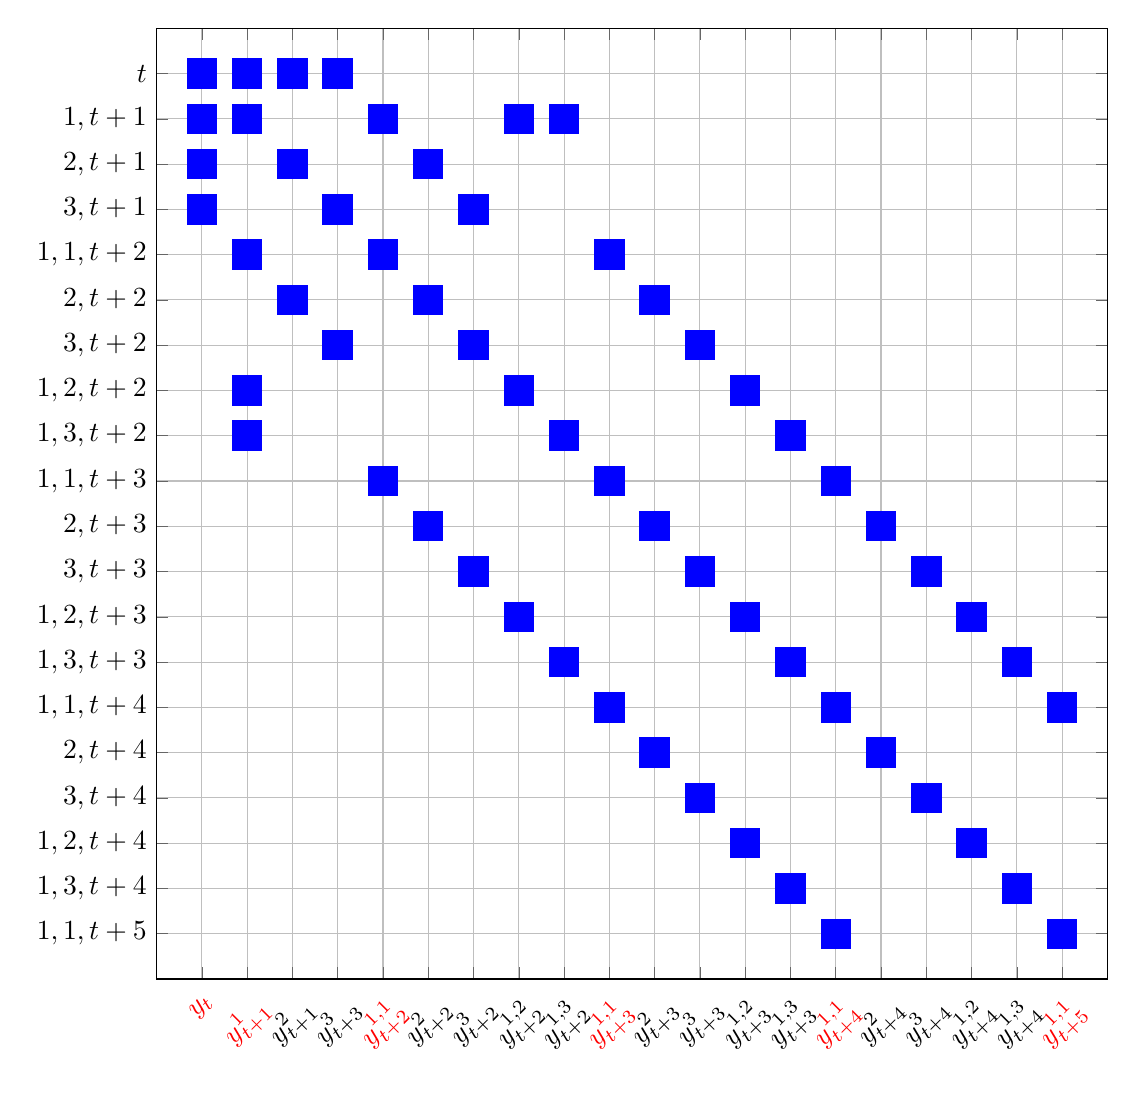
\begin{tikzpicture}

\begin{axis}[%
width=4.754in,
height=4.754in,
at={(1.648in,0.642in)},
scale only axis,
xmin=0,
xmax=21,
xtick={1,2,3,4,5,6,7,8,9,10,11,12,13,14,15,16,17,18,19,20},
xticklabels={{\color{red}$y_{t}$},{\color{red}$y_{t+1}^1$},{$y_{t+1}^2$},{$y_{t+3}^3$},{\color{red}$y_{t+2}^{1,1}$},{$y_{t+2}^2$},{$y_{t+2}^3$},{$y_{t+2}^{1,2}$},{$y_{t+2}^{1,3}$},{\color{red}$y_{t+3}^{1,1}$},{$y_{t+3}^2$},{$y_{t+3}^3$},{$y_{t+3}^{1,2}$},{$y_{t+3}^{1,3}$},{\color{red}$y_{t+4}^{1,1}$},{$y_{t+4}^2$},{$y_{t+4}^3$},{$y_{t+4}^{1,2}$},{$y_{t+4}^{1,3}$},{\color{red}$y_{t+5}^{1,1}$}},
xticklabel style={rotate=45},
y dir=reverse,
ymin=0,
ymax=21,
ytick={1,2,3,4,5,6,7,8,9,10,11,12,13,14,15,16,17,18,19,20},
yticklabels={{$t$},{$1,t+1$},{$2,t+1$},{$3,t+1$},{$1,1,t+2$},{$2,t+2$},{$3,t+2$},{$1,2,t+2$},{$1,3,t+2$},{$1,1,t+3$},{$2,t+3$},{$3,t+3$},{$1,2,t+3$},{$1,3,t+3$},{$1,1,t+4$},{$2,t+4$},{$3,t+4$},{$1,2,t+4$},{$1,3,t+4$},{$1,1,t+5$}},
axis background/.style={fill=white},
xmajorgrids,
ymajorgrids
]
\addplot [color=blue, only marks, mark size=5.3pt, mark=square*, mark options={solid, blue}, forget plot]
  table[row sep=crcr]
   \end{center}

\end{frame}


\begin{frame}
   \frametitle{Burnside (1998) asset pricing model}

   \begin{itemize}

      \item The price/dividend ratio and the growth rate of dividends:
            \[
               \begin{split}
                  y_t & = \beta \mathbb E_t\left[e^{\theta x_{t+1}}\left(1+y_{t+1}\right)\right] \\
                  x_t & = (1-\rho)\bar x + \rho x_{t-1}+\epsilon_t
               \end{split}
            \]

      \item The exact solution is:
            \[
               y_t = \sum_{i=1}^\infty \beta^i e^{a_i+b_i\hat x_t}
            \]
            where
            \[
               a_i = \theta \bar x i +
               \frac{\theta^2\sigma^2}{2(1-\rho)^2}\left(i-2\rho\frac{1-\rho^i}{1-\rho}+\rho^2\frac{1-\rho^{2i}}{1-\rho^2}\right)
            \]
            and
            \[
               b_i = \frac{\theta\rho\left(1-\rho^i\right)}{1-\rho}
            \]

   \end{itemize}

\end{frame}


\begin{frame}
   \frametitle{Numerical simulation}
   \framesubtitle{Calibration}

   \begin{align*}
      \bar x & = 0.0179  \\
      \rho   & =  -0.139 \\
      \theta & = -1.5    \\
      \beta  & = 0.95    \\
      \sigma & = 0.0348  \\
   \end{align*}

   \medskip

   \begin{itemize}
      \item The deterministic steady state is equal to 12.3035.\newline
      \item The risky steady state, defined as the fix point in absence of
            shock this period:
            \[
               \widetilde y = \sum_{i=1}^\infty \beta^i e^{\theta \bar x i +
                     \frac{\theta^2\sigma^2}{2(1-\rho)^2}\left(i-2\rho\frac{1-\rho^i}{1-\rho}+\rho^2\frac{1-\rho^{2i}}{1-\rho^2}\right)}\approx 12.4812
            \]

   \end{itemize}

\end{frame}

\begin{frame}
   \frametitle{Comparing SEP, perturbation and closed-form solution}

   Simulate long time series ($T=8000$) and compare with true solution. We use a quadrature with 3 nodes for SEP.\newline

   \bigskip

   \begin{tabular}{l|cc|cc}
      \hline
                                                     & P(1)   & P(2)   & SEP(0) & SEP(2) \\ \hline
      $100\times\textrm{mean}(|\hat y_t - y_t|/y_t)$ & 1.4261 & 0.0193 & 1.4241 & 1.2534 \\
      $100\times\textrm{max}(|\hat y_t - y_t|/y_t)$  & 1.4707 & 0.0527 & 1.4250 & 1.2539 \\ \hline\hline
   \end{tabular}

   \bigskip\bigskip

   One can show, using the closed for solution and considering an infinite number of weights and nodes in the quadrature, that we would have to consider an approximation order greater than 60, to be able to recover the theoretical mean of the price-dividend ratio.


\end{frame}



\begin{frame}
   \frametitle{Hybrid approach}

   \begin{itemize}

      \item Consider a Taylor expansion of the original problem only along the scale $\sigma$ of the shocks\newline

      \item Use the second order correction for the constant.\newline

      \item[$\Rightarrow$] For K-order SEP, replace $y_{t+K+1}$ in the equations in period $K$ by $y_{t+K+1}+\frac{1}{2}g_{\sigma\sigma}$.\newline

   \end{itemize}

   \bigskip

   \scalebox{.9}{
      \begin{tabular}{l|c|ccc}
         \hline
                                                        & P(2)   & SEP(2) & SEP(2+) & SEP(10+) \\ \hline
         $100\times\textrm{mean}(|\hat y_t - y_t|/y_t)$ & 0.0193 & 1.2534 & 0.0165  & 0.0153   \\
         $100\times\textrm{max}(|\hat y_t - y_t|/y_t)$  & 0.0527 & 1.2539 & 0.0179  & 0.0170   \\ \hline\hline
      \end{tabular}}

\end{frame}


\begin{frame}
   \frametitle{Irreversible investment}
   Consider the following RBC model with irreversible investment:
   \[
      \begin{split}
         \max_{\{c_{t+j},l_{t+j},k_{t+j+1}\}_{j=0}^{\infty}} & \quad \mathcal W_t = \sum_{j=0}^{\infty}\beta^ju(c_{t+j},l_{t+j}) \\
         \underline{s.t.}                                    &                                                                   \\
         \qquad y_t                                          & = c_t + i_t                                                       \\
         \qquad y_t                                          & = A_tf(k_{t},l_t)                                                 \\
         \qquad k_{t+1}                                      & = i_t + (1-\delta)k_{t}                                           \\
         \qquad A_{t}                                        & = {A^{\star}}e^{a_{t}}                                            \\
         \qquad a_{t}                                        & = \rho a_{t-1} + \varepsilon_t                                    \\
         \qquad i_t                                          & \ge 0
      \end{split}
   \]
\end{frame}

\begin{frame}
   \frametitle{Further specifications}
   The utility function is
   \[
      u(c_t,l_t) = \frac{\left(c_t^{\theta}(1-l_t)^{1-\theta}\right)^{\tau}}{1-\tau}
   \]
   and the production function,
   \[
      f(k_{t},l_t) = \left(\alpha k_{t}^{\psi} + (1-\alpha)l_t^{\psi}\right)^{\frac{1}{\psi}}
   \]
\end{frame}

\begin{frame}
   \frametitle{First order conditions}
   {\footnotesize\[
         \begin{split}
            u_c(c_t,l_t) - \mu_t                & = \beta \mathbb E_t\Big[
            u_c(c_{t+1},l_{t+1})\Bigl(A_{t+1}f_k(k_{t+1},l_{t+1}) + 1
            -\delta\Bigr) - \mu_{t+1}(1-\delta)\Big]                                               \\
            \frac{u_{l}(c_t,l_t)}{u_c(c_t,l_t)} & = A_tf_l(k_t,l_t)                                \\
            c_t + k_{t+1}                       & = A_tf(k_{t},l_t) + (1-\delta)k_{t}              \\
            0                                   & = \mu_t \left( k_{t+1} - (1-\delta)k_{t} \right)
         \end{split}
      \]}

   \bigskip\bigskip

   where $\mu_t$ is the Lagrange multiplier associated with the constraint on investment.
\end{frame}

\begin{frame}
   \frametitle{Calibration}
   \begin{align*}
      \beta   & =  0.990 \\
      \theta  & =  0.357 \\
      \tau    & =  2.000 \\
      \alpha  & =  0.450 \\
      \psi    & = -0.500 \\
      \delta  & =  0.010 \\
      \rho    & =  0.800 \\
      A^\star & =  1.000 \\
      \sigma  & =  0.100
   \end{align*}
\end{frame}


\begin{frame}
   \frametitle{Simulation of the RBC model}
   \framesubtitle{SEP with orders=0,\dots,10}
   \begin{center}
      \scalebox{.5}{
         % This file was created by matlab2tikz.
%
%The latest updates can be retrieved from
%  http://www.mathworks.com/matlabcentral/fileexchange/22022-matlab2tikz-matlab2tikz
%where you can also make suggestions and rate matlab2tikz.
%
\begin{tikzpicture}

\begin{axis}[%
width=31in,
height=17.293in,
at={(5.2in,2.334in)},
scale only axis,
xmin=1,
xmax=101,
ymin=-0.772194981575012,
ymax=1.65088355541229,
ylabel style={font=\color{white!15!black}},
ylabel={Investment},
axis background/.style={fill=white}
]
\addplot [color=black, forget plot]
  table[row sep=crcr]{%
1	0.177702040741409\\
2	0.283678871039512\\
3	0.677124839756\\
4	0.0824838016040463\\
5	0.267863391883711\\
6	0.311717571374166\\
7	0.0299523950325569\\
8	-0.0157257598187055\\
9	0.0832350956043056\\
10	0.929403649185556\\
11	1.62986695278717\\
12	0.829309708082963\\
13	1.65088357931634\\
14	1.51773699481356\\
15	1.12710990490289\\
16	1.09470509002036\\
17	0.768849068343392\\
18	0.555385346426013\\
19	0.868947240413064\\
20	1.1211005312356\\
21	1.34413428881577\\
22	1.23963275687048\\
23	0.527635342381533\\
24	0.602658485501459\\
25	0.968755548588764\\
26	0.875690999351196\\
27	0.99327364723098\\
28	0.975802803657732\\
29	0.607895596454025\\
30	0.526533842556063\\
31	0.156692748648538\\
32	0.339884246926735\\
33	-0.0539016910897502\\
34	-0.291183556431799\\
35	-0.400342222857126\\
36	-0.771753968678463\\
37	-0.427860590450035\\
38	-0.288819685173124\\
39	-0.368873043272288\\
40	-0.0251893339851559\\
41	-0.348627708816667\\
42	-0.293900324183002\\
43	-0.272473930519342\\
44	-0.151336923981497\\
45	-0.0499391622283409\\
46	-0.195438439604021\\
47	-0.149900754743346\\
48	-0.137109993578671\\
49	0.0282365061130419\\
50	0.278059838075542\\
51	0.505772946870918\\
52	0.193564365730039\\
53	0.18159373428265\\
54	-0.0930779308524565\\
55	-0.255262920409649\\
56	-0.188685256158933\\
57	0.16848404502026\\
58	-0.00637627390945751\\
59	0.0888555295256731\\
60	0.0445221354652518\\
61	0.295674761249941\\
62	0.02209736090604\\
63	0.0451173623301892\\
64	0.170828191695544\\
65	0.405317539123375\\
66	0.736837253638717\\
67	0.605618145248462\\
68	0.131603728070541\\
69	-0.0274427336119491\\
70	-0.192454758864626\\
71	0.34529850346805\\
72	0.15234966827331\\
73	0.305545475705741\\
74	0.215044646508763\\
75	0.393091169537992\\
76	0.152618360465427\\
77	-0.129666789779723\\
78	-0.311903255143949\\
79	-0.150632756753247\\
80	-0.125920045604308\\
81	-0.108215366215278\\
82	0.212828607558224\\
83	0.255962831129138\\
84	0.269921891164909\\
85	0.61618370401211\\
86	0.307901017443087\\
87	0.426026400168026\\
88	0.560369498334128\\
89	0.39486852797867\\
90	0.379290893982794\\
91	0.064741536736263\\
92	-0.138322687553492\\
93	-0.0684456440312267\\
94	0.108063251687653\\
95	0.726216540339417\\
96	0.410285036702758\\
97	0.384673652038145\\
98	0.30089466552351\\
99	-0.12678726759874\\
100	-0.153951324691752\\
101	-0.371786880503129\\
};
\addplot [color=black!90!red, forget plot]
  table[row sep=crcr]{%
1	0.177702040741409\\
2	0.283577070429264\\
3	0.677068866261963\\
4	0.0823531930551832\\
5	0.267757050802386\\
6	0.311616480466256\\
7	0.0298217125539757\\
8	-0.015856277866384\\
9	0.0831200480878621\\
10	0.929378619634448\\
11	1.62989478605484\\
12	0.829234000293023\\
13	1.65086790820188\\
14	1.51768144580654\\
15	1.12700172514281\\
16	1.09458088214931\\
17	0.768692244690182\\
18	0.555210945955073\\
19	0.868788289503828\\
20	1.12094791850825\\
21	1.3439815895878\\
22	1.23946070001786\\
23	0.527424187833048\\
24	0.602449989579327\\
25	0.968558089126592\\
26	0.875484350327404\\
27	0.993065608787103\\
28	0.975588182280523\\
29	0.60766799649838\\
30	0.526304745786761\\
31	0.156460389474168\\
32	0.339658685016799\\
33	-0.0541265422371268\\
34	-0.291401146760157\\
35	-0.400550077373085\\
36	-0.771946387530969\\
37	-0.428045180953002\\
38	-0.288994702612987\\
39	-0.36903948978819\\
40	-0.0253459112919449\\
41	-0.348779547273684\\
42	-0.294043532057004\\
43	-0.272609129112825\\
44	-0.151464029949949\\
45	-0.0500594844515075\\
46	-0.195554666019784\\
47	-0.150010273167126\\
48	-0.137213601984486\\
49	0.0281397130276311\\
50	0.277968779012265\\
51	0.505684250880114\\
52	0.193469877053171\\
53	0.181500462513357\\
54	-0.0931715648472367\\
55	-0.255352582684154\\
56	-0.188767963933155\\
57	0.16840987307041\\
58	-0.0064508214785495\\
59	0.0887851356796234\\
60	0.0444533724532019\\
61	0.295610901542469\\
62	0.0220300967258902\\
63	0.0450531112329556\\
64	0.17076758754364\\
65	0.405259973083656\\
66	0.736780384389107\\
67	0.605552685343263\\
68	0.131529165120158\\
69	-0.0275168827423948\\
70	-0.192526475508229\\
71	0.345236841672257\\
72	0.152284683342732\\
73	0.305482874584346\\
74	0.214980191082026\\
75	0.393028452770243\\
76	0.152551384059886\\
77	-0.129734802300731\\
78	-0.311967910962975\\
79	-0.150689272608268\\
80	-0.125971598096434\\
81	-0.108262431575561\\
82	0.21278939753892\\
83	0.255923659023438\\
84	0.269881801758991\\
85	0.616146597178698\\
86	0.307853911630215\\
87	0.425979136697646\\
88	0.560320582945591\\
89	0.394812607313418\\
90	0.379232272388099\\
91	0.0646773389518749\\
92	-0.13838678650696\\
93	-0.068504247218187\\
94	0.108010510124984\\
95	0.726172720345419\\
96	0.410229807819034\\
97	0.384615362411725\\
98	0.30083313182062\\
99	-0.126854302000933\\
100	-0.154013978606668\\
101	-0.371847010462909\\
};
\addplot [color=black!80!red, forget plot]
  table[row sep=crcr]{%
1	0.177702040741409\\
2	0.283508883696199\\
3	0.677018091639969\\
4	0.0822721738183644\\
5	0.267686575113669\\
6	0.311548157007622\\
7	0.0297419858135179\\
8	-0.0159347741014789\\
9	0.0830489603425323\\
10	0.92933950281869\\
11	1.62986587255507\\
12	0.829167693483451\\
13	1.65081384208249\\
14	1.51760842495678\\
15	1.12690857869407\\
16	1.09447919304528\\
17	0.768579121871077\\
18	0.555092127407933\\
19	0.868671632027759\\
20	1.12082909525352\\
21	1.34385743484279\\
22	1.23932781036823\\
23	0.527283593141484\\
24	0.602309515113128\\
25	0.968416524426506\\
26	0.875339343835899\\
27	0.992917332294075\\
28	0.975436414576657\\
29	0.607515886227016\\
30	0.526153327995637\\
31	0.156313605533946\\
32	0.339512956177127\\
33	-0.0542650434862112\\
34	-0.291531386440332\\
35	-0.400672448116279\\
36	-0.772054018690977\\
37	-0.428151875567691\\
38	-0.289097230492694\\
39	-0.369135196291698\\
40	-0.0254409765163212\\
41	-0.348866160666291\\
42	-0.294125309489845\\
43	-0.272685999788333\\
44	-0.151537780132822\\
45	-0.0501307657421062\\
46	-0.195620605804678\\
47	-0.15007271131774\\
48	-0.137272475369222\\
49	0.0280819177589158\\
50	0.277909107661495\\
51	0.505620579016313\\
52	0.193409944862218\\
53	0.181441574754679\\
54	-0.0932249796024157\\
55	-0.255400354071911\\
56	-0.188812441332461\\
57	0.168363346132066\\
58	-0.0064937358953448\\
59	0.0887427857320747\\
60	0.0444130379883106\\
61	0.295567822984792\\
62	0.0219911892051255\\
63	0.0450156154809217\\
64	0.170729525192265\\
65	0.405218047040853\\
66	0.736730059002288\\
67	0.605500713010855\\
68	0.131483143555496\\
69	-0.0275591959787991\\
70	-0.192563885235827\\
71	0.34519388178749\\
72	0.152244247429461\\
73	0.305440289472608\\
74	0.214938606125494\\
75	0.392983612106824\\
76	0.15250963970331\\
77	-0.129771123283643\\
78	-0.31199854892841\\
79	-0.150717690269347\\
80	-0.125997306589145\\
81	-0.108285599063819\\
82	0.212763782729823\\
83	0.255896970189657\\
84	0.26985417282745\\
85	0.61611150551386\\
86	0.307820920558745\\
87	0.425942987330833\\
88	0.560279832015082\\
89	0.394771898167214\\
90	0.379190276338609\\
91	0.0646393421650771\\
92	-0.138420382579915\\
93	-0.0685357364600946\\
94	0.107978811853813\\
95	0.726130441373704\\
96	0.410189122312991\\
97	0.384573426934089\\
98	0.300791257688278\\
99	-0.126890028903956\\
100	-0.154046317632117\\
101	-0.371873557323758\\
};
\addplot [color=black!70!red, forget plot]
  table[row sep=crcr]{%
1	0.177702040741409\\
2	0.283463716096715\\
3	0.676978436837078\\
4	0.0822216395105795\\
5	0.267640251406545\\
6	0.311502616151349\\
7	0.0296929828786155\\
8	-0.0159823920513329\\
9	0.0830047603273753\\
10	0.929303688825186\\
11	1.62982680384185\\
12	0.829116815230738\\
13	1.65075982038627\\
14	1.51754496120137\\
15	1.12683790515061\\
16	1.0944037929511\\
17	0.768500556179761\\
18	0.555012452549209\\
19	0.868589829167975\\
20	1.1207431928853\\
21	1.3437658859086\\
22	1.23923221388593\\
23	0.527190738952695\\
24	0.602215993083724\\
25	0.968318643931696\\
26	0.875240341484909\\
27	0.992815174739157\\
28	0.975332333958435\\
29	0.60741516308839\\
30	0.526053774388324\\
31	0.156220296366419\\
32	0.339418717849919\\
33	-0.0543511619745239\\
34	-0.291610319439205\\
35	-0.40074547143106\\
36	-0.772114799445741\\
37	-0.428214422761562\\
38	-0.289158183101958\\
39	-0.369191028658468\\
40	-0.0254994533462737\\
41	-0.348916194529927\\
42	-0.294172692507635\\
43	-0.272730431506906\\
44	-0.151581311051416\\
45	-0.0501737177403814\\
46	-0.195658595329794\\
47	-0.150108878098267\\
48	-0.137306474806296\\
49	0.0280469168149762\\
50	0.277870074378817\\
51	0.505576369546676\\
52	0.193371682718511\\
53	0.181404063999885\\
54	-0.0932559550121445\\
55	-0.255426016492137\\
56	-0.188836631513631\\
57	0.168333908989594\\
58	-0.00651887977022691\\
59	0.088716922261742\\
60	0.0443889685970523\\
61	0.295539039718259\\
62	0.0219682844355496\\
63	0.0449933492080413\\
64	0.170705416553032\\
65	0.405188618236568\\
66	0.736691151485592\\
67	0.605462511995442\\
68	0.131454436904972\\
69	-0.027583744847707\\
70	-0.192583484077177\\
71	0.345164559405854\\
72	0.152218845543615\\
73	0.305411687398053\\
74	0.214911727162812\\
75	0.392952512738236\\
76	0.152483394547735\\
77	-0.129790704010778\\
78	-0.312012508374278\\
79	-0.150731910520148\\
80	-0.126010047134243\\
81	-0.108296896236182\\
82	0.212747029074187\\
83	0.255878986350766\\
84	0.269835415547633\\
85	0.616083519552661\\
86	0.307798307438345\\
87	0.425916878721585\\
88	0.560249111993264\\
89	0.394743345461808\\
90	0.379161114860933\\
91	0.0646165167711254\\
92	-0.138438071513324\\
93	-0.0685528490886094\\
94	0.107959493959729\\
95	0.726096550445538\\
96	0.410160385557057\\
97	0.384544232918888\\
98	0.30076314365229\\
99	-0.126909227443897\\
100	-0.154063018661711\\
101	-0.371884170518498\\
};
\addplot [color=black!60!red, forget plot]
  table[row sep=crcr]{%
1	0.177702040741409\\
2	0.283434037152432\\
3	0.67694958633445\\
4	0.082189972264224\\
5	0.267609989486646\\
6	0.311472561079977\\
7	0.0296626630456759\\
8	-0.0160115127061847\\
9	0.0829771314131289\\
10	0.929275643069728\\
11	1.62979245350009\\
12	0.829080196408805\\
13	1.65071639225708\\
14	1.51749663374323\\
15	1.12678743154176\\
16	1.09435062187303\\
17	0.768447252716063\\
18	0.554959628292222\\
19	0.868533992070869\\
20	1.12068349553265\\
21	1.34370157821827\\
22	1.23916598917051\\
23	0.527129782472445\\
24	0.602154271845606\\
25	0.96825241831352\\
26	0.875173886467666\\
27	0.99274620850186\\
28	0.975262272393517\\
29	0.607348913967075\\
30	0.525988647087405\\
31	0.15616075713457\\
32	0.339357787141077\\
33	-0.0544055484627297\\
34	-0.291658916436153\\
35	-0.400789477482046\\
36	-0.772149390270324\\
37	-0.428251502933179\\
38	-0.289194829923859\\
39	-0.369223980674871\\
40	-0.025535731631913\\
41	-0.34894545923474\\
42	-0.294200484774559\\
43	-0.272756384773954\\
44	-0.151607289121529\\
45	-0.0501998418023506\\
46	-0.195680821806294\\
47	-0.150130161581552\\
48	-0.137326359622748\\
49	0.0280253787249391\\
50	0.277844630940624\\
51	0.505546330358239\\
52	0.193347219230371\\
53	0.181380163796404\\
54	-0.0932741193029581\\
55	-0.255439895471302\\
56	-0.188849915466598\\
57	0.168315190117056\\
58	-0.00653381339621137\\
59	0.0887009680148454\\
60	0.0443744238094031\\
61	0.295519983130397\\
62	0.0219546176767149\\
63	0.044979954070392\\
64	0.170690084597406\\
65	0.405168468904046\\
66	0.736662986979321\\
67	0.605435623852331\\
68	0.131436393636073\\
69	-0.0275981802290713\\
70	-0.192593780872381\\
71	0.345144853035417\\
72	0.152202802320795\\
73	0.305392680283788\\
74	0.214894365411094\\
75	0.392931393325157\\
76	0.152466812182756\\
77	-0.129801351119333\\
78	-0.312018465005218\\
79	-0.150738967046962\\
80	-0.126016294459939\\
81	-0.108302319115371\\
82	0.212736094694533\\
83	0.255866993953075\\
84	0.269822843830292\\
85	0.616062889646426\\
86	0.307783059565479\\
87	0.42589867311049\\
88	0.560227155455956\\
89	0.394723807853944\\
90	0.379141292942036\\
91	0.0646026481724168\\
92	-0.138447428547624\\
93	-0.0685622499884617\\
94	0.107947598331767\\
95	0.726071535818964\\
96	0.410140633425172\\
97	0.384524357482496\\
98	0.300744469787127\\
99	-0.126919626950897\\
100	-0.154071643612329\\
101	-0.371887568645549\\
};
\addplot [color=black!50!red, forget plot]
  table[row sep=crcr]{%
1	0.177702040741409\\
2	0.283414652099377\\
3	0.676929422678064\\
4	0.0821700498889693\\
5	0.267590312222802\\
6	0.311452870269701\\
7	0.0296437933861371\\
8	-0.0160294531553401\\
9	0.082959783036222\\
10	0.929255222250677\\
11	1.62976610989932\\
12	0.82905478744713\\
13	1.65068445104024\\
14	1.51746205769895\\
15	1.12675259402016\\
16	1.09431420492022\\
17	0.768411610361084\\
18	0.554924937382039\\
19	0.868496530879457\\
20	1.12064297973724\\
21	1.34365764599642\\
22	1.23912113193534\\
23	0.527089975768944\\
24	0.602113796297842\\
25	0.968208233602184\\
26	0.875129782480125\\
27	0.992700258635449\\
28	0.975215680345899\\
29	0.607305560676803\\
30	0.525946188729597\\
31	0.156122683194766\\
32	0.339318419677031\\
33	-0.0544396936009965\\
34	-0.291688860686865\\
35	-0.40081650281831\\
36	-0.772169233964396\\
37	-0.428273706201273\\
38	-0.28921707559263\\
39	-0.369243635198968\\
40	-0.0255583860655905\\
41	-0.348962764397841\\
42	-0.294216968601248\\
43	-0.272771728022371\\
44	-0.151622967701886\\
45	-0.0502158876129558\\
46	-0.195693932702146\\
47	-0.150142786384432\\
48	-0.137338185664469\\
49	0.028012098762571\\
50	0.277828097013342\\
51	0.505526220640586\\
52	0.193331554701011\\
53	0.181364893349068\\
54	-0.0932849858073311\\
55	-0.255447456824135\\
56	-0.188857283893584\\
57	0.16830327055186\\
58	-0.00654278699537895\\
59	0.0886910458975772\\
60	0.0443655440469727\\
61	0.295507448329062\\
62	0.0219463694551988\\
63	0.0449718087722767\\
64	0.170680311603829\\
65	0.405154906954173\\
66	0.73664335328559\\
67	0.605417200484508\\
68	0.131425020299077\\
69	-0.0276067707256319\\
70	-0.192599208417673\\
71	0.345131760225551\\
72	0.152192631502549\\
73	0.305380154557899\\
74	0.214883161777733\\
75	0.392917259623256\\
76	0.152456306660671\\
77	-0.129807194597335\\
78	-0.312020714939856\\
79	-0.150742429828477\\
80	-0.126019313954845\\
81	-0.108304864807895\\
82	0.2127289777366\\
83	0.255859064385347\\
84	0.269814501852734\\
85	0.616048339586383\\
86	0.307772902003552\\
87	0.425886267125747\\
88	0.560211960450548\\
89	0.394710663488942\\
90	0.379128019404383\\
91	0.0645941431888734\\
92	-0.138452403956106\\
93	-0.0685674731955584\\
94	0.107940215194195\\
95	0.726053891130304\\
96	0.410127304010773\\
97	0.384511029430983\\
98	0.30073216904432\\
99	-0.126925309524022\\
100	-0.154076097170549\\
101	-0.371887949669848\\
};
\addplot [color=black!40!red, forget plot]
  table[row sep=crcr]{%
1	0.177702040741409\\
2	0.283402047718417\\
3	0.676915680392963\\
4	0.082157475189797\\
5	0.267577562970969\\
6	0.311440039934104\\
7	0.0296319905154313\\
8	-0.0160405785729406\\
9	0.0829488488219914\\
10	0.929240948252419\\
11	1.62974717497514\\
12	0.82903755814163\\
13	1.65066202472589\\
14	1.51743816995571\\
15	1.12672905493353\\
16	1.09428972162179\\
17	0.768388054933812\\
18	0.554902168892356\\
19	0.868471692815281\\
20	1.12061590161153\\
21	1.34362815432339\\
22	1.23909118652365\\
23	0.527064078910857\\
24	0.602087383466345\\
25	0.968179036863523\\
26	0.875100745653606\\
27	0.992669920218351\\
28	0.975184956164047\\
29	0.607277303102138\\
30	0.525918592293694\\
31	0.156098307067793\\
32	0.339293008758767\\
33	-0.0544613038606883\\
34	-0.291707480512975\\
35	-0.400832734582199\\
36	-0.772180710590271\\
37	-0.428287170073496\\
38	-0.289230684902388\\
39	-0.36925546666085\\
40	-0.0255725999049186\\
41	-0.348973098250461\\
42	-0.294226842047918\\
43	-0.272780890884646\\
44	-0.151632515212083\\
45	-0.0502258079808273\\
46	-0.195701759158427\\
47	-0.150150365434857\\
48	-0.1373452461011\\
49	0.0280038366998645\\
50	0.277817384703739\\
51	0.505512902330437\\
52	0.193321522106455\\
53	0.181355129958682\\
54	-0.093291490854769\\
55	-0.255451610113581\\
56	-0.188861418582958\\
57	0.168295666646564\\
58	-0.00654824528468759\\
59	0.0886848439374207\\
60	0.0443600740532027\\
61	0.295499257913343\\
62	0.0219413434001578\\
63	0.0449668118348064\\
64	0.170674076173502\\
65	0.405145889934454\\
66	0.736629988619842\\
67	0.605404801157908\\
68	0.131417823200597\\
69	-0.027611950265208\\
70	-0.192602079870304\\
71	0.345123136093813\\
72	0.152186171492201\\
73	0.305371953435709\\
74	0.214875945341601\\
75	0.39290790184148\\
76	0.152449616879094\\
77	-0.129810432947682\\
78	-0.312021337847777\\
79	-0.150744102863771\\
80	-0.126020743531897\\
81	-0.108306020328073\\
82	0.212724359026477\\
83	0.255853857605259\\
84	0.269809010474484\\
85	0.616038356449568\\
86	0.307766197818281\\
87	0.425877947121212\\
88	0.560201664355061\\
89	0.394701928214125\\
90	0.379119227506543\\
91	0.0645888886926917\\
92	-0.138455064978538\\
93	-0.0685704089722589\\
94	0.107935605369774\\
95	0.726041788224543\\
96	0.410118426800013\\
97	0.384502195503312\\
98	0.300724118876471\\
99	-0.126928443902538\\
100	-0.154078396382397\\
101	-0.371887251957874\\
};
\addplot [color=black!30!red, forget plot]
  table[row sep=crcr]{%
1	0.177702040741409\\
2	0.283393880469029\\
3	0.676906470722908\\
4	0.0821495165978717\\
5	0.267569325632168\\
6	0.311431714447065\\
7	0.0296245761525129\\
8	-0.0160475176072845\\
9	0.0829419357388454\\
10	0.929231221335991\\
11	1.62973405356358\\
12	0.829026054380382\\
13	1.65064670890485\\
14	1.51742202031097\\
15	1.12671337377469\\
16	1.09427346650303\\
17	0.768372600121405\\
18	0.554887395426478\\
19	0.868455360183419\\
20	1.12059799278438\\
21	1.34360858660043\\
22	1.23907139252357\\
23	0.527047282025068\\
24	0.60207021114554\\
25	0.96815987518474\\
26	0.875081738552048\\
27	0.992650017905315\\
28	0.97516481749401\\
29	0.607258940949569\\
30	0.525900698124152\\
31	0.156082689044027\\
32	0.33927662108192\\
33	-0.0544750181691988\\
34	-0.291719118516634\\
35	-0.400843192448458\\
36	-0.772187384903339\\
37	-0.428295341757475\\
38	-0.289239048261403\\
39	-0.369262631659917\\
40	-0.0255815358619167\\
41	-0.348979310115679\\
42	-0.294232795000288\\
43	-0.272786400017165\\
44	-0.151638361318462\\
45	-0.0502319461895391\\
46	-0.195706464062372\\
47	-0.150154945711211\\
48	-0.137349502376134\\
49	0.0279986800089741\\
50	0.277810469884046\\
51	0.505504158068071\\
52	0.193315106306327\\
53	0.181348893874357\\
54	-0.0932954265135334\\
55	-0.255453901677596\\
56	-0.188863750954222\\
57	0.168290819669211\\
58	-0.0065515732117733\\
59	0.0886809565515294\\
60	0.044356692520243\\
61	0.295493935105427\\
62	0.0219382608898879\\
63	0.0449637292671832\\
64	0.170670095662661\\
65	0.405139953707796\\
66	0.736621039711213\\
67	0.605396564117058\\
68	0.13141326467273\\
69	-0.0276150828104293\\
70	-0.192603599877702\\
71	0.345117497017388\\
72	0.152182066351324\\
73	0.30536661533968\\
74	0.21487130715316\\
75	0.392901758982752\\
76	0.152445372172921\\
77	-0.129812242053543\\
78	-0.31202130673381\\
79	-0.150744889961922\\
80	-0.126021396619709\\
81	-0.108306513961676\\
82	0.212721372539684\\
83	0.255850460421328\\
84	0.269805420788068\\
85	0.616031633841574\\
86	0.30776180827564\\
87	0.42587243323232\\
88	0.560194790651877\\
89	0.394696177163451\\
90	0.379113453350387\\
91	0.0645856242082872\\
92	-0.138456495198587\\
93	-0.0685720762315546\\
94	0.107932716003411\\
95	0.726033640181365\\
96	0.410112572762031\\
97	0.384496389894913\\
98	0.300718879111844\\
99	-0.126930188104635\\
100	-0.154079581199845\\
101	-0.371886312240348\\
};
\addplot [color=black!20!red, forget plot]
  table[row sep=crcr]{%
1	0.177702040741409\\
2	0.283388602466121\\
3	0.676900370796534\\
4	0.082144468091453\\
5	0.267564014631645\\
6	0.311426329309997\\
7	0.0296199018446821\\
8	-0.0160518669463257\\
9	0.0829375536538365\\
10	0.929224704251714\\
11	1.6297251654956\\
12	0.829018456280639\\
13	1.65063643203749\\
14	1.51741125799351\\
15	1.12670303031718\\
16	1.09426276950266\\
17	0.768362517833442\\
18	0.554877819472452\\
19	0.868444686384833\\
20	1.12058623720483\\
21	1.34359571015925\\
22	1.23905840134316\\
23	0.527036414930935\\
24	0.602059080077731\\
25	0.968147363604679\\
26	0.875069351427603\\
27	0.992637024324725\\
28	0.975151675907495\\
29	0.607247039091897\\
30	0.525889118897202\\
31	0.156072679809966\\
32	0.339266062821827\\
33	-0.0544837377192898\\
34	-0.291726421812949\\
35	-0.400849523247751\\
36	-0.772191305709565\\
37	-0.428300354275157\\
38	-0.289244218075279\\
39	-0.369267006243094\\
40	-0.0255871720806316\\
41	-0.348983078989691\\
42	-0.294236417260368\\
43	-0.272789744181147\\
44	-0.151641968368922\\
45	-0.0502358366909009\\
46	-0.195709319108541\\
47	-0.150157738685018\\
48	-0.137352092155634\\
49	0.0279954458963064\\
50	0.277806013443223\\
51	0.505498449006929\\
52	0.193311004917441\\
53	0.181344908348678\\
54	-0.0932978289264782\\
55	-0.25545517941242\\
56	-0.188865083600246\\
57	0.168287726937476\\
58	-0.00655362237931898\\
59	0.0886785097585604\\
60	0.0443545877167708\\
61	0.295490487110851\\
62	0.0219363572648545\\
63	0.0449618283964281\\
64	0.170667556556972\\
65	0.405136070523727\\
66	0.736615113777303\\
67	0.605391140263154\\
68	0.131410371129057\\
69	-0.0276169982922658\\
70	-0.192604409505476\\
71	0.345113827198964\\
72	0.152179453683688\\
73	0.305363153490287\\
74	0.214868328566986\\
75	0.392897749677481\\
76	0.152442670662909\\
77	-0.12981326463287\\
78	-0.312021065194835\\
79	-0.15074524890167\\
80	-0.126021681454471\\
81	-0.108306705345127\\
82	0.212719444870392\\
83	0.255848252714243\\
84	0.269803084768757\\
85	0.616027164281095\\
86	0.307758945425119\\
87	0.425868809126969\\
88	0.560190248893904\\
89	0.394692415735847\\
90	0.379109683772827\\
91	0.0645835977210384\\
92	-0.138457270679601\\
93	-0.0685730353308333\\
94	0.107930897501719\\
95	0.726028224389858\\
96	0.41010873924762\\
97	0.384492597820604\\
98	0.300715481570101\\
99	-0.126931169863726\\
100	-0.154080192407155\\
101	-0.37188545626642\\
};
\addplot [color=black!10!red, forget plot]
  table[row sep=crcr]{%
1	0.177702040741409\\
2	0.283385198611774\\
3	0.676896364717463\\
4	0.0821412601389951\\
5	0.26756059619177\\
6	0.311422854641583\\
7	0.0296169459849892\\
8	-0.0160546045150706\\
9	0.0829347703680381\\
10	0.929220389202496\\
11	1.62971923558554\\
12	0.829013477104454\\
13	1.65062961987344\\
14	1.51740415735692\\
15	1.12669625642912\\
16	1.09425577556404\\
17	0.76835596885551\\
18	0.55487163024805\\
19	0.868437742958547\\
20	1.12057856340993\\
21	1.34358728780966\\
22	1.23904991924192\\
23	0.527029398484359\\
24	0.602051882110141\\
25	0.968139225848976\\
26	0.875061305878283\\
27	0.992628572689629\\
28	0.975143131082175\\
29	0.607239340362209\\
30	0.525881638744101\\
31	0.156066264766762\\
32	0.339259266411969\\
33	-0.0544892891838964\\
34	-0.291731019951594\\
35	-0.400853473196478\\
36	-0.772193624529673\\
37	-0.428303444649106\\
38	-0.2892474203493\\
39	-0.369269688676936\\
40	-0.0255907288879773\\
41	-0.348985378151993\\
42	-0.294238633135837\\
43	-0.272791785637442\\
44	-0.151644202675123\\
45	-0.0502382516817066\\
46	-0.195711063176682\\
47	-0.150159452464609\\
48	-0.137353678223486\\
49	0.0279934120489336\\
50	0.277803147305269\\
51	0.505494739583981\\
52	0.193308390338031\\
53	0.181342362202062\\
54	-0.0932993047452151\\
55	-0.255455897869314\\
56	-0.18886585244123\\
57	0.168285753900731\\
58	-0.00655489088319006\\
59	0.0886769662664456\\
60	0.0443532724137164\\
61	0.295488260728367\\
62	0.0219351758967016\\
63	0.0449606231874895\\
64	0.170665936645788\\
65	0.405133544412715\\
66	0.736611222501559\\
67	0.605387593588412\\
68	0.131408533345257\\
69	-0.0276181764222321\\
70	-0.192604843168919\\
71	0.345111449261089\\
72	0.152177790674381\\
73	0.305360916402557\\
74	0.214866418713825\\
75	0.392895145759418\\
76	0.152440951000549\\
77	-0.129813848140689\\
78	-0.31202079527974\\
79	-0.150745403467517\\
80	-0.126021794885285\\
81	-0.108306763665585\\
82	0.212718203659051\\
83	0.255846823631208\\
84	0.26980157101633\\
85	0.616024220780857\\
86	0.307757089460043\\
87	0.425866442695027\\
88	0.560187271410855\\
89	0.394689968755968\\
90	0.379107234935295\\
91	0.0645823095487096\\
92	-0.13845769379046\\
93	-0.068573592618742\\
94	0.10792975060211\\
95	0.726024658524107\\
96	0.410106243287868\\
97	0.384490133659052\\
98	0.300713286306697\\
99	-0.126931727790978\\
100	-0.154080506994194\\
101	-0.371884776590278\\
};
\addplot [color=red, forget plot]
  table[row sep=crcr]{%
1	0.177702040741409\\
2	0.283383006978088\\
3	0.676893750214512\\
4	0.0821392183092054\\
5	0.267558398810495\\
6	0.311420616980976\\
7	0.0296150721873708\\
8	-0.016056333637607\\
9	0.0829329992831334\\
10	0.929217555921151\\
11	1.62971532095698\\
12	0.829010233181591\\
13	1.6506251431587\\
14	1.51739950639188\\
15	1.12669184389357\\
16	1.09425122495284\\
17	0.768351729201835\\
18	0.554867639125222\\
19	0.868433242254594\\
20	1.12057357518534\\
21	1.34358180293172\\
22	1.23904440341508\\
23	0.527024875821293\\
24	0.602047236517623\\
25	0.96813394871189\\
26	0.875056094183635\\
27	0.992623091070364\\
28	0.97513759000562\\
29	0.60723436894071\\
30	0.525876813647093\\
31	0.15606215389535\\
32	0.339254895310199\\
33	-0.0544928268963495\\
34	-0.291733922502473\\
35	-0.400855946987625\\
36	-0.772195006292556\\
37	-0.428305359549087\\
38	-0.289249488152678\\
39	-0.36927140246746\\
40	-0.0255930395697585\\
41	-0.348986783265066\\
42	-0.294239991053532\\
43	-0.272793034300712\\
44	-0.151645587542303\\
45	-0.0502397658066372\\
46	-0.195712130742263\\
47	-0.150160505919719\\
48	-0.137354651425804\\
49	0.027992133517748\\
50	0.277801309843034\\
51	0.505492341645543\\
52	0.193306735519748\\
53	0.181340738905448\\
54	-0.0933002134378276\\
55	-0.2554563023864\\
56	-0.188866297406116\\
57	0.168284497757966\\
58	-0.00655567727408299\\
59	0.0886759931535119\\
60	0.0443524500401753\\
61	0.295486828686322\\
62	0.0219344415329754\\
63	0.0449598785879434\\
64	0.170664904890226\\
65	0.405131909133683\\
66	0.736608683984991\\
67	0.605385287422226\\
68	0.131407366735669\\
69	-0.0276189035990932\\
70	-0.192605074006756\\
71	0.345109914495767\\
72	0.152176733036358\\
73	0.305359475668298\\
74	0.214865196547774\\
75	0.392893461792566\\
76	0.152439857082221\\
77	-0.129814184986388\\
78	-0.312020561664186\\
79	-0.150745462462477\\
80	-0.126021830990764\\
81	-0.108306767109517\\
82	0.21271740672831\\
83	0.255845902089309\\
84	0.269800594567457\\
85	0.616022296370335\\
86	0.307755890453884\\
87	0.425864905752165\\
88	0.560185331400441\\
89	0.394688383995746\\
90	0.37910565068315\\
91	0.0645815075855416\\
92	-0.13845792627679\\
93	-0.0685739196405269\\
94	0.107929025950231\\
95	0.72602232706054\\
96	0.410104625367773\\
97	0.384488538761192\\
98	0.300711871805817\\
99	-0.126932048001657\\
100	-0.154080668492374\\
101	-0.371884273749689\\
};
\addplot [color=blue, dashed, line width=2.0pt, forget plot]
  table[row sep=crcr]{%
1	0.177702040741409\\
101	0.177702040741409\\
};
\end{axis}

\begin{axis}[%
width=40in,
height=21.219in,
at={(0in,0in)},
scale only axis,
xmin=0,
xmax=1,
ymin=0,
ymax=1,
axis line style={draw=none},
ticks=none,
axis x line*=bottom,
axis y line*=left
]
\end{axis}
\end{tikzpicture}%}
   \end{center}

\end{frame}


\begin{frame}
   \frametitle{Simulation of the RBC model (irreversible investment)}
   \framesubtitle{SEP with orders=0,\dots,5}
   \begin{center}
      \scalebox{.5}{
         % This file was created by matlab2tikz.
%
%The latest updates can be retrieved from
%  http://www.mathworks.com/matlabcentral/fileexchange/22022-matlab2tikz-matlab2tikz
%where you can also make suggestions and rate matlab2tikz.
%
\definecolor{mycolor1}{rgb}{0.00000,1.00000,1.00000}%
\definecolor{mycolor2}{rgb}{1.00000,0.00000,1.00000}%
%
\begin{tikzpicture}

\begin{axis}[%
width=6.781in,
height=5.348in,
at={(1.137in,0.722in)},
scale only axis,
xmin=1,
xmax=101,
ymin=0,
ymax=1.65178634897904,
ylabel style={font=\color{white!15!black}},
ylabel={Investment},
axis background/.style={fill=white},
legend style={legend cell align=left, align=left, draw=white!15!black}
]
\addplot [color=black, line width=2.0pt]
  table[row sep=crcr]{%
1	0.177702040741409\\
2	0.283678871040422\\
3	0.677124853607844\\
4	0.0824838012783184\\
5	0.267863391672896\\
6	0.311717502450485\\
7	0.029952398321226\\
8	0\\
9	0.0829062661862932\\
10	0.929303023068924\\
11	1.62993679374562\\
12	0.829168309992099\\
13	1.65091844029842\\
14	1.51772330338239\\
15	1.12701008831555\\
16	1.09459561508234\\
17	0.768684967617267\\
18	0.555191631655365\\
19	0.868803078334877\\
20	1.12099270893083\\
21	1.34405448006444\\
22	1.24574125718373\\
23	0.527362446935885\\
24	0.602404557670976\\
25	0.983884399548912\\
26	0.895445696117527\\
27	1.0249614985743\\
28	1.01578338968848\\
29	0.644639798088267\\
30	0.56458978714503\\
31	0.195154173615623\\
32	0.375606722403737\\
33	0.011426513556819\\
34	0\\
35	0\\
36	0\\
37	0\\
38	0\\
39	0\\
40	0\\
41	0\\
42	0\\
43	0\\
44	0\\
45	0\\
46	0\\
47	0\\
48	0\\
49	0\\
50	0.206912758260623\\
51	0.446325986384799\\
52	0.122858913259821\\
53	0.112422666773611\\
54	0\\
55	0\\
56	0\\
57	0.0920177891448049\\
58	0\\
59	0.011594070835933\\
60	0\\
61	0.230954610167834\\
62	0\\
63	0\\
64	0.105162150840503\\
65	0.351010667395535\\
66	0.697319916241752\\
67	0.561591796942152\\
68	0.0714783607376064\\
69	0\\
70	0\\
71	0.29145837619945\\
72	0.092956919383731\\
73	0.253298190701511\\
74	0.161126885973881\\
75	0.346750552117695\\
76	0.0996759714893127\\
77	0\\
78	0\\
79	0\\
80	0\\
81	0\\
82	0.149898089002856\\
83	0.196681721393148\\
84	0.212919289393949\\
85	0.574966821096584\\
86	0.255401629883033\\
87	0.379439471754418\\
88	0.519929489313191\\
89	0.349505058551844\\
90	0.334615957567779\\
91	0.0112869833712896\\
92	0\\
93	0\\
94	0.0540510420156426\\
95	0.694846264794482\\
96	0.368882272245936\\
97	0.343559601687789\\
98	0.258363941289546\\
99	0\\
100	0\\
101	0\\
};
\addlegendentry{order=0}

\addplot [color=blue]
  table[row sep=crcr]{%
1	0.177702040741409\\
2	0.300761817238588\\
3	0.676881035322861\\
4	0.127495254170008\\
5	0.284683729560755\\
6	0.326013129175456\\
7	0.0788428045927627\\
8	0.0381275116873489\\
9	0.124866433452121\\
10	0.927819449031557\\
11	1.63092158803682\\
12	0.82706157833067\\
13	1.65136935188604\\
14	1.51744900875229\\
15	1.12546509102668\\
16	1.09289917875416\\
17	0.766183449165493\\
18	0.552253866507524\\
19	0.866583545592543\\
20	1.11995796554535\\
21	1.34649608076897\\
22	1.24835535075456\\
23	0.534799452597965\\
24	0.607473914799403\\
25	0.98543572924309\\
26	0.897815651320131\\
27	1.02678086685194\\
28	1.01828615181477\\
29	0.650436153070957\\
30	0.575073904460406\\
31	0.252154891476104\\
32	0.407749578607478\\
33	0.0898017948888745\\
34	0.0164438106451092\\
35	0\\
36	0\\
37	0\\
38	0\\
39	0\\
40	0.0681117903625863\\
41	0\\
42	0\\
43	0\\
44	0.0211613921163292\\
45	0.0468116052971943\\
46	0.00174778893469085\\
47	0.0167505358964546\\
48	0.0171504739568578\\
49	0.0628220730225133\\
50	0.246277837311223\\
51	0.454057133729556\\
52	0.175063423609477\\
53	0.164963941982203\\
54	0.0288731586179249\\
55	0\\
56	0\\
57	0.143934615686223\\
58	0.0456380019371685\\
59	0.0754148804910108\\
60	0.0613860656362135\\
61	0.258300586553547\\
62	0.0522360885943402\\
63	0.0642563148042232\\
64	0.146501697112415\\
65	0.359279202238604\\
66	0.683995715250124\\
67	0.547052793643154\\
68	0.121623973559258\\
69	0.0438107636106251\\
70	0\\
71	0.308193714081061\\
72	0.135786573358104\\
73	0.27486393567591\\
74	0.193560518623753\\
75	0.354145849432735\\
76	0.139943358247126\\
77	0.0109334954315852\\
78	0\\
79	0.00100154827092602\\
80	0.00600592689758072\\
81	0.0131040429355376\\
82	0.180613916932607\\
83	0.219234550463182\\
84	0.233586962041477\\
85	0.558637792519523\\
86	0.272011322128613\\
87	0.38033505508214\\
88	0.50672322294401\\
89	0.357429234694096\\
90	0.343882340200353\\
91	0.0649792912666111\\
92	0.00623347835765964\\
93	0.0270833363938914\\
94	0.0991974561931245\\
95	0.679830961253177\\
96	0.37197441054154\\
97	0.35135854884323\\
98	0.274500443905994\\
99	0.0127201830244901\\
100	0.00132130221751447\\
101	0\\
};
\addlegendentry{order=1}

\addplot [color=mycolor1]
  table[row sep=crcr]{%
1	0.177702040741409\\
2	0.312363535468877\\
3	0.676702254107105\\
4	0.154137788396576\\
5	0.296159891295702\\
6	0.336221847239974\\
7	0.107103418582403\\
8	0.0686807699831362\\
9	0.149779548773147\\
10	0.926812377426849\\
11	1.63147527045349\\
12	0.825664941221664\\
13	1.65158832009963\\
14	1.51721162601823\\
15	1.12442789167937\\
16	1.09176791076736\\
17	0.764546232655816\\
18	0.559780592043406\\
19	0.865022729073747\\
20	1.1192217401345\\
21	1.34868955901108\\
22	1.25000446736987\\
23	0.552107480115708\\
24	0.620999022929578\\
25	0.987898871560956\\
26	0.901454542602012\\
27	1.02996476622708\\
28	1.02119825971069\\
29	0.664288454153203\\
30	0.59384909386226\\
31	0.293964056026845\\
32	0.438115753371675\\
33	0.138494933948789\\
34	0.0179730444214228\\
35	0\\
36	0\\
37	0\\
38	0\\
39	0\\
40	0.106415674835447\\
41	0\\
42	0\\
43	0\\
44	0.024357671220949\\
45	0.0709779331016356\\
46	0\\
47	0.0155765518773743\\
48	0.0179566611977335\\
49	0.0982137322709781\\
50	0.279523616110176\\
51	0.471032143738487\\
52	0.211104054377548\\
53	0.201690933048751\\
54	0.0387832717251009\\
55	0\\
56	0\\
57	0.180446972053508\\
58	0.0710951693201462\\
59	0.118020937927589\\
60	0.0932402412345885\\
61	0.284911045410003\\
62	0.0819903724304649\\
63	0.0932905783325557\\
64	0.181517486748944\\
65	0.376956529871418\\
66	0.678584457316284\\
67	0.553032382683017\\
68	0.154829196092543\\
69	0.0622915641080801\\
70	0\\
71	0.327287056516688\\
72	0.170291524851922\\
73	0.294658100368522\\
74	0.222369772600672\\
75	0.371162083772933\\
76	0.1736755781056\\
77	0.00827869683357418\\
78	0\\
79	0\\
80	0\\
81	0.00828199081373282\\
82	0.207706753079689\\
83	0.245239936885617\\
84	0.257420720949016\\
85	0.555322946244066\\
86	0.292918859342987\\
87	0.393136672343116\\
88	0.510238045188302\\
89	0.370198928080869\\
90	0.358857387673024\\
91	0.108406957056159\\
92	0\\
93	0.0351349756876309\\
94	0.127907536808232\\
95	0.670598733484969\\
96	0.38407471157468\\
97	0.363970485147374\\
98	0.295810357141819\\
99	0.0070999982284825\\
100	0\\
101	0\\
};
\addlegendentry{order=2}

\addplot [color=mycolor2]
  table[row sep=crcr]{%
1	0.177702040741409\\
2	0.320150626542793\\
3	0.676576509302551\\
4	0.170283777897713\\
5	0.30421899089516\\
6	0.343306335503784\\
7	0.123894273212757\\
8	0.0865163879281307\\
9	0.164959960556096\\
10	0.926168581070989\\
11	1.63178260045715\\
12	0.824785001463284\\
13	1.65169217471279\\
14	1.51703779784045\\
15	1.12376779139208\\
16	1.0910509799189\\
17	0.768174689963319\\
18	0.570586317883419\\
19	0.86733003119562\\
20	1.11861301474818\\
21	1.34998851834362\\
22	1.25203925792093\\
23	0.569622523701714\\
24	0.637815486953711\\
25	0.993496407238528\\
26	0.909721270578386\\
27	1.03503024966628\\
28	1.02688700426357\\
29	0.681047739984294\\
30	0.612491097326455\\
31	0.322284510571346\\
32	0.462129747470173\\
33	0.168749108481137\\
34	0.0230071273289918\\
35	0\\
36	0\\
37	0\\
38	0\\
39	0\\
40	0.130567677969462\\
41	0\\
42	0\\
43	0\\
44	0.0297071418210097\\
45	0.0878822626507329\\
46	0\\
47	0.0193103489945729\\
48	0.0223000772109851\\
49	0.121794813254912\\
50	0.301037918300028\\
51	0.487392306532769\\
52	0.23713776855326\\
53	0.227245833447838\\
54	0.0477277973021204\\
55	0\\
56	0\\
57	0.207439916375051\\
58	0.0874617429940212\\
59	0.147187208463223\\
60	0.117586627719436\\
61	0.304019987424648\\
62	0.102726993219542\\
63	0.113372670178651\\
64	0.201917569569957\\
65	0.391758030661213\\
66	0.682796091913215\\
67	0.562759322317173\\
68	0.180991370691665\\
69	0.076224303094289\\
70	0\\
71	0.345782773683825\\
72	0.189793058582534\\
73	0.31473693305071\\
74	0.241368580534322\\
75	0.385924022227085\\
76	0.192348267056184\\
77	0.0105844125157071\\
78	0\\
79	0\\
80	0\\
81	0.00776501946197116\\
82	0.222866782377284\\
83	0.259572254291227\\
84	0.272137820154509\\
85	0.561456883304337\\
86	0.306685678112024\\
87	0.405190048938704\\
88	0.518310664361427\\
89	0.383951019192395\\
90	0.372317773039387\\
91	0.126710343768228\\
92	0\\
93	0.0395315608189337\\
94	0.151897510785351\\
95	0.672275978762813\\
96	0.397089241160593\\
97	0.377419194045383\\
98	0.310297806933476\\
99	0.00916630417810671\\
100	0\\
101	0\\
};
\addlegendentry{order=3}

\addplot [color=green]
  table[row sep=crcr]{%
1	0.177702040741409\\
2	0.32533097301555\\
3	0.676504878736959\\
4	0.180105733968127\\
5	0.310391195167714\\
6	0.34859092565881\\
7	0.134045960226058\\
8	0.0971517719157371\\
9	0.174315961193581\\
10	0.925749895465973\\
11	1.63196338557404\\
12	0.825936291100253\\
13	1.65174814679314\\
14	1.51691347792015\\
15	1.12435610245109\\
16	1.09271759161836\\
17	0.774652621152037\\
18	0.580968290957275\\
19	0.873207373326354\\
20	1.12236804855903\\
21	1.35283029324021\\
22	1.25644676622752\\
23	0.585139136108465\\
24	0.651807395497477\\
25	1.00257255581102\\
26	0.920078283309899\\
27	1.04409863389847\\
28	1.03647295406841\\
29	0.695552434909196\\
30	0.629453371043327\\
31	0.342433208422451\\
32	0.481919363048077\\
33	0.187799865139137\\
34	0.0279172808992294\\
35	0\\
36	0\\
37	0\\
38	0\\
39	0\\
40	0.146671753310933\\
41	0\\
42	0\\
43	0\\
44	0.0357024924667959\\
45	0.0987760043408454\\
46	0\\
47	0.0241251911748879\\
48	0.027997243148399\\
49	0.136280111876889\\
50	0.318029016603176\\
51	0.502302022382199\\
52	0.256481362991278\\
53	0.247042304676943\\
54	0.0537616353671089\\
55	0\\
56	0\\
57	0.222964053904698\\
58	0.0976889943670942\\
59	0.16275053739878\\
60	0.131104163639335\\
61	0.316935160005611\\
62	0.114918495259294\\
63	0.128180461793758\\
64	0.216038840222609\\
65	0.403984570505078\\
66	0.690096041887973\\
67	0.573756188481209\\
68	0.19716914378205\\
69	0.0847648058718482\\
70	0\\
71	0.357090280730415\\
72	0.206774785429782\\
73	0.325510121945014\\
74	0.255194671105243\\
75	0.397766950819866\\
76	0.209347379324695\\
77	0.0120893172341192\\
78	0\\
79	0\\
80	0.00201275192076444\\
81	0.0100085091811231\\
82	0.238605145960371\\
83	0.27202236054076\\
84	0.283524731024647\\
85	0.568487397315508\\
86	0.319218390774117\\
87	0.416225579551358\\
88	0.528849264962014\\
89	0.394990127788504\\
90	0.384365288911756\\
91	0.141424068087992\\
92	0.00190347145308056\\
93	0.0450847555007718\\
94	0.164835949497275\\
95	0.677526573168052\\
96	0.407910328995448\\
97	0.388636219458179\\
98	0.323682353981406\\
99	0.0121436243151121\\
100	0\\
101	0\\
};
\addlegendentry{order=4}

\addplot [color=red]
  table[row sep=crcr]{%
1	0.177702040741409\\
2	0.328903060851707\\
3	0.678800081420151\\
4	0.186171805736631\\
5	0.314882856203594\\
6	0.352680923586379\\
7	0.140224714004446\\
8	0.103569562161666\\
9	0.180096942453904\\
10	0.926161204194752\\
11	1.63208510784421\\
12	0.82819083502446\\
13	1.65178634897904\\
14	1.51742214707229\\
15	1.12749743332023\\
16	1.09635355269556\\
17	0.781161858914291\\
18	0.588886557984506\\
19	0.879241939867461\\
20	1.12765155302326\\
21	1.35811591674937\\
22	1.26307848310696\\
23	0.597275508686011\\
24	0.662847119317719\\
25	1.01162978569858\\
26	0.929936442411299\\
27	1.05309533884233\\
28	1.04589868414735\\
29	0.708020849692559\\
30	0.641518103740408\\
31	0.356844794558067\\
32	0.494513249900173\\
33	0.200327851654758\\
34	0.0322542876997021\\
35	0\\
36	0\\
37	0\\
38	0\\
39	0\\
40	0.156805282544082\\
41	0\\
42	0\\
43	0\\
44	0.0407708586422433\\
45	0.106188669069305\\
46	0.00171496688099482\\
47	0.0278143805307367\\
48	0.0326170948581634\\
49	0.144748863970502\\
50	0.330817710196351\\
51	0.512700381535334\\
52	0.267414160107469\\
53	0.2579036881991\\
54	0.0582922704132751\\
55	0\\
56	0\\
57	0.232637733832658\\
58	0.105078400597791\\
59	0.171803513239536\\
60	0.13852039136386\\
61	0.328809071735712\\
62	0.121540001705527\\
63	0.136513318014999\\
64	0.227867158290283\\
65	0.413034548798028\\
66	0.697014761232125\\
67	0.581135601864793\\
68	0.206875821453857\\
69	0.0913022657241946\\
70	0\\
71	0.366974267830061\\
72	0.217908514772061\\
73	0.336437647755389\\
74	0.267245179849641\\
75	0.406862168744479\\
76	0.219791063376011\\
77	0.0144770613395519\\
78	0\\
79	0\\
80	0.00405573043783769\\
81	0.0126109592854002\\
82	0.248907167130264\\
83	0.283145922720321\\
84	0.294651063853656\\
85	0.577268407247628\\
86	0.3288975741562\\
87	0.423827080620909\\
88	0.534861372382482\\
89	0.403207575677497\\
90	0.392189441904105\\
91	0.150987692267775\\
92	0.00333356135006224\\
93	0.0492910454867163\\
94	0.172251184841905\\
95	0.682050310880021\\
96	0.415420630163593\\
97	0.396677741227159\\
98	0.330008185138058\\
99	0.0138302794790672\\
100	0\\
101	0\\
};
\addlegendentry{order=5}

\addplot [color=blue, dashed, line width=2.0pt, forget plot]
  table[row sep=crcr]
   \end{center}

\end{frame}


\begin{frame}
   \frametitle{Simulation of the RBC model (irreversible investment)}
   \framesubtitle{SEP with orders=0,\dots,10}
   \begin{center}
      \scalebox{.5}{
         % This file was created by matlab2tikz.
%
%The latest updates can be retrieved from
%  http://www.mathworks.com/matlabcentral/fileexchange/22022-matlab2tikz-matlab2tikz
%where you can also make suggestions and rate matlab2tikz.
%
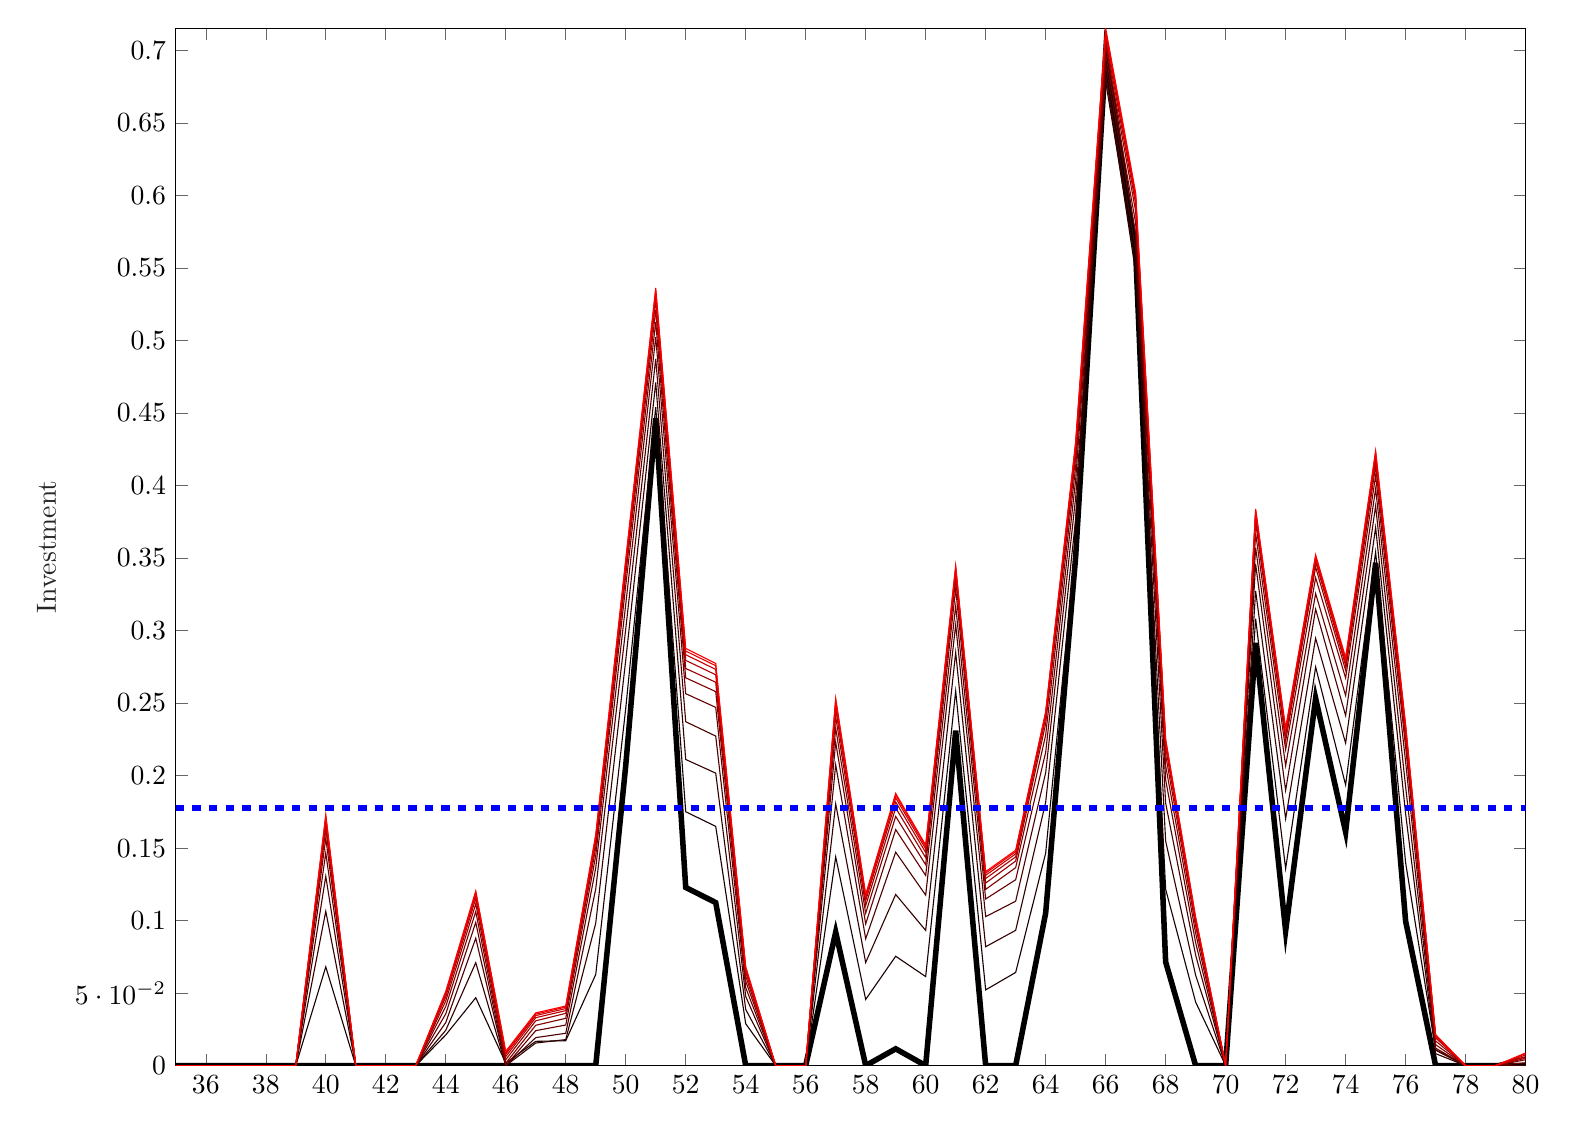
\begin{tikzpicture}

\begin{axis}[%
width=6.749in,
height=5.187in,
at={(1.132in,0.7in)},
scale only axis,
xmin=35,
xmax=80,
ymin=0,
ymax=0.715361118899045,
ylabel style={font=\color{white!15!black}},
ylabel={Investment},
axis background/.style={fill=white}
]
\addplot [color=black, line width=2.0pt, forget plot]
  table[row sep=crcr]{%
35	0\\
36	0\\
37	0\\
38	0\\
39	0\\
40	0\\
41	0\\
42	0\\
43	0\\
44	0\\
45	0\\
46	0\\
47	0\\
48	0\\
49	0\\
50	0.206912758260623\\
51	0.446325986384799\\
52	0.122858913259821\\
53	0.112422666773611\\
54	0\\
55	0\\
56	0\\
57	0.0920177891448049\\
58	0\\
59	0.011594070835933\\
60	0\\
61	0.230954610167834\\
62	0\\
63	0\\
64	0.105162150840503\\
65	0.351010667395535\\
66	0.697319916241752\\
67	0.561591796942152\\
68	0.0714783607376064\\
69	0\\
70	0\\
71	0.29145837619945\\
72	0.092956919383731\\
73	0.253298190701511\\
74	0.161126885973881\\
75	0.346750552117695\\
76	0.0996759714893127\\
77	0\\
78	0\\
79	0\\
80	0\\
};
\addplot [color=black!90!red, forget plot]
  table[row sep=crcr]{%
35	0\\
36	0\\
37	0\\
38	0\\
39	0\\
40	0.0681117903625863\\
41	0\\
42	0\\
43	0\\
44	0.0211613921163292\\
45	0.0468116052971943\\
46	0.00174778893469085\\
47	0.0167505358964546\\
48	0.0171504739568578\\
49	0.0628220730225133\\
50	0.246277837311223\\
51	0.454057133729556\\
52	0.175063423609477\\
53	0.164963941982203\\
54	0.0288731586179249\\
55	0\\
56	0\\
57	0.143934615686223\\
58	0.0456380019371685\\
59	0.0754148804910108\\
60	0.0613860656362135\\
61	0.258300586553547\\
62	0.0522360885943402\\
63	0.0642563148042232\\
64	0.146501697112415\\
65	0.359279202238604\\
66	0.683995715250124\\
67	0.547052793643154\\
68	0.121623973559258\\
69	0.0438107636106251\\
70	0\\
71	0.308193714081061\\
72	0.135786573358104\\
73	0.27486393567591\\
74	0.193560518623753\\
75	0.354145849432735\\
76	0.139943358247126\\
77	0.0109334954315852\\
78	0\\
79	0.00100154827092602\\
80	0.00600592689758072\\
};
\addplot [color=black!80!red, forget plot]
  table[row sep=crcr]{%
35	0\\
36	0\\
37	0\\
38	0\\
39	0\\
40	0.106415674835447\\
41	0\\
42	0\\
43	0\\
44	0.024357671220949\\
45	0.0709779331016356\\
46	0\\
47	0.0155765518773743\\
48	0.0179566611977335\\
49	0.0982137322709781\\
50	0.279523616110176\\
51	0.471032143738487\\
52	0.211104054377548\\
53	0.201690933048751\\
54	0.0387832717251009\\
55	0\\
56	0\\
57	0.180446972053508\\
58	0.0710951693201462\\
59	0.118020937927589\\
60	0.0932402412345885\\
61	0.284911045410003\\
62	0.0819903724304649\\
63	0.0932905783325557\\
64	0.181517486748944\\
65	0.376956529871418\\
66	0.678584457316284\\
67	0.553032382683017\\
68	0.154829196092543\\
69	0.0622915641080801\\
70	0\\
71	0.327287056516688\\
72	0.170291524851922\\
73	0.294658100368522\\
74	0.222369772600672\\
75	0.371162083772933\\
76	0.1736755781056\\
77	0.00827869683357418\\
78	0\\
79	0\\
80	0\\
};
\addplot [color=black!70!red, forget plot]
  table[row sep=crcr]{%
35	0\\
36	0\\
37	0\\
38	0\\
39	0\\
40	0.130567677969462\\
41	0\\
42	0\\
43	0\\
44	0.0297071418210097\\
45	0.0878822626507329\\
46	0\\
47	0.0193103489945729\\
48	0.0223000772109851\\
49	0.121794813254912\\
50	0.301037918300028\\
51	0.487392306532769\\
52	0.23713776855326\\
53	0.227245833447838\\
54	0.0477277973021204\\
55	0\\
56	0\\
57	0.207439916375051\\
58	0.0874617429940212\\
59	0.147187208463223\\
60	0.117586627719436\\
61	0.304019987424648\\
62	0.102726993219542\\
63	0.113372670178651\\
64	0.201917569569957\\
65	0.391758030661213\\
66	0.682796091913215\\
67	0.562759322317173\\
68	0.180991370691665\\
69	0.076224303094289\\
70	0\\
71	0.345782773683825\\
72	0.189793058582534\\
73	0.31473693305071\\
74	0.241368580534322\\
75	0.385924022227085\\
76	0.192348267056184\\
77	0.0105844125157071\\
78	0\\
79	0\\
80	0\\
};
\addplot [color=black!60!red, forget plot]
  table[row sep=crcr]{%
35	0\\
36	0\\
37	0\\
38	0\\
39	0\\
40	0.146671753310933\\
41	0\\
42	0\\
43	0\\
44	0.0357024924667959\\
45	0.0987760043408454\\
46	0\\
47	0.0241251911748879\\
48	0.027997243148399\\
49	0.136280111876889\\
50	0.318029016603176\\
51	0.502302022382199\\
52	0.256481362991278\\
53	0.247042304676943\\
54	0.0537616353671089\\
55	0\\
56	0\\
57	0.222964053904698\\
58	0.0976889943670942\\
59	0.16275053739878\\
60	0.131104163639335\\
61	0.316935160005611\\
62	0.114918495259294\\
63	0.128180461793758\\
64	0.216038840222609\\
65	0.403984570505078\\
66	0.690096041887973\\
67	0.573756188481209\\
68	0.19716914378205\\
69	0.0847648058718482\\
70	0\\
71	0.357090280730415\\
72	0.206774785429782\\
73	0.325510121945014\\
74	0.255194671105243\\
75	0.397766950819866\\
76	0.209347379324695\\
77	0.0120893172341192\\
78	0\\
79	0\\
80	0.00201275192076444\\
};
\addplot [color=black!50!red, forget plot]
  table[row sep=crcr]{%
35	0\\
36	0\\
37	0\\
38	0\\
39	0\\
40	0.156805282544082\\
41	0\\
42	0\\
43	0\\
44	0.0407708586422433\\
45	0.106188669069305\\
46	0.00171496688099482\\
47	0.0278143805307367\\
48	0.0326170948581634\\
49	0.144748863970502\\
50	0.330817710196351\\
51	0.512700381535334\\
52	0.267414160107469\\
53	0.2579036881991\\
54	0.0582922704132751\\
55	0\\
56	0\\
57	0.232637733832658\\
58	0.105078400597791\\
59	0.171803513239536\\
60	0.13852039136386\\
61	0.328809071735712\\
62	0.121540001705527\\
63	0.136513318014999\\
64	0.227867158290283\\
65	0.413034548798028\\
66	0.697014761232125\\
67	0.581135601864793\\
68	0.206875821453857\\
69	0.0913022657241946\\
70	0\\
71	0.366974267830061\\
72	0.217908514772061\\
73	0.336437647755389\\
74	0.267245179849641\\
75	0.406862168744479\\
76	0.219791063376011\\
77	0.0144770613395519\\
78	0\\
79	0\\
80	0.00405573043783769\\
};
\addplot [color=black!40!red, forget plot]
  table[row sep=crcr]{%
35	0\\
36	0\\
37	0\\
38	0\\
39	0\\
40	0.16313999990383\\
41	0\\
42	0\\
43	0\\
44	0.0446181696475938\\
45	0.111471169215879\\
46	0.00409999395808902\\
47	0.0309134592287361\\
48	0.0360351047074721\\
49	0.150194462656308\\
50	0.33813302237664\\
51	0.520963821800648\\
52	0.273874681479601\\
53	0.264375892426975\\
54	0.0617791778645535\\
55	0\\
56	0\\
57	0.240485313501495\\
58	0.110320102225508\\
59	0.17765600306589\\
60	0.14341492657476\\
61	0.335999332185346\\
62	0.125885365660744\\
63	0.141092910282964\\
64	0.23582332632736\\
65	0.419752322871557\\
66	0.703247801163574\\
67	0.589100759247454\\
68	0.214321281191051\\
69	0.0960710058380955\\
70	0\\
71	0.37452101378913\\
72	0.22366795095235\\
73	0.34368077712592\\
74	0.272605666126184\\
75	0.413541253511453\\
76	0.225125427404395\\
77	0.0170056142715214\\
78	0\\
79	0\\
80	0.00505602069957911\\
};
\addplot [color=black!30!red, forget plot]
  table[row sep=crcr]{%
35	0\\
36	0\\
37	0\\
38	0\\
39	0\\
40	0.167106633140723\\
41	0\\
42	0\\
43	0\\
44	0.0474068035601009\\
45	0.115222224235801\\
46	0.00621326584703019\\
47	0.0330521860924273\\
48	0.0379466803977728\\
49	0.153903751673674\\
50	0.342567131833056\\
51	0.527413519205792\\
52	0.279431096747759\\
53	0.269534512872381\\
54	0.064464213757504\\
55	0\\
56	0\\
57	0.245944125315474\\
58	0.113772459955472\\
59	0.181788270882988\\
60	0.146974091256365\\
61	0.339810732425141\\
62	0.129009586130059\\
63	0.143934130326027\\
64	0.239728818653802\\
65	0.424078831734667\\
66	0.70746191740563\\
67	0.594326956063375\\
68	0.219434715754488\\
69	0.0987954211360202\\
70	0\\
71	0.37860148373816\\
72	0.226806608296756\\
73	0.347323250675835\\
74	0.27588800771343\\
75	0.417586343632361\\
76	0.228727854403403\\
77	0.0190873318372542\\
78	0\\
79	0\\
80	0.00600729683528844\\
};
\addplot [color=black!20!red, forget plot]
  table[row sep=crcr]{%
35	0\\
36	0\\
37	0\\
38	0\\
39	0\\
40	0.169962364787538\\
41	0\\
42	0\\
43	0\\
44	0.0492572621046447\\
45	0.11769929439943\\
46	0.00786386236738789\\
47	0.0345066825826126\\
48	0.0393439735382426\\
49	0.156394485509749\\
50	0.345434255142012\\
51	0.531621196009331\\
52	0.283353478930727\\
53	0.273215401771478\\
54	0.0663232055037659\\
55	0\\
56	0\\
57	0.249486570269065\\
58	0.11585459285615\\
59	0.184614121543195\\
60	0.149398525888008\\
61	0.342053294515015\\
62	0.131198579663252\\
63	0.146012816133238\\
64	0.241957817213452\\
65	0.426977147533611\\
66	0.711118527392388\\
67	0.597661867808498\\
68	0.222636359640798\\
69	0.100601499795512\\
70	0\\
71	0.380954565942905\\
72	0.229339958317151\\
73	0.349360797519566\\
74	0.277964845214992\\
75	0.420599050758286\\
76	0.231864534311277\\
77	0.020268730525538\\
78	0\\
79	0\\
80	0.00727348087991375\\
};
\addplot [color=black!10!red, forget plot]
  table[row sep=crcr]{%
35	0\\
36	0\\
37	0\\
38	0\\
39	0\\
40	0.171754039392575\\
41	0\\
42	0\\
43	0\\
44	0.0503797527646557\\
45	0.119467524317999\\
46	0.0090473167315479\\
47	0.0355124377090945\\
48	0.0403539542536082\\
49	0.158132511646645\\
50	0.347545973602497\\
51	0.53451812252946\\
52	0.285885742581521\\
53	0.275770557553196\\
54	0.0674876738314587\\
55	0\\
56	0\\
57	0.251799535841536\\
58	0.117208647256008\\
59	0.186484128855344\\
60	0.151026359580838\\
61	0.34356877009719\\
62	0.132733112855797\\
63	0.147511553702\\
64	0.243213266029993\\
65	0.42907897059573\\
66	0.713515957044485\\
67	0.600039380584835\\
68	0.224262732580199\\
69	0.101645463698508\\
70	0\\
71	0.38262094674385\\
72	0.231327629635072\\
73	0.350979415322803\\
74	0.279884412095189\\
75	0.422627242444269\\
76	0.233977738992102\\
77	0.0209295810047918\\
78	0\\
79	0\\
80	0.00821650206871016\\
};
\addplot [color=red, forget plot]
  table[row sep=crcr]{%
35	0\\
36	0\\
37	0\\
38	0\\
39	0\\
40	0.172857147597689\\
41	0\\
42	0\\
43	0\\
44	0.0511981633671694\\
45	0.120414815350031\\
46	0.00988874687401652\\
47	0.0363732749912582\\
48	0.0410795750627948\\
49	0.159266049313152\\
50	0.349092388353274\\
51	0.536199621222013\\
52	0.287665730745454\\
53	0.277353792515928\\
54	0.0682028962300156\\
55	0\\
56	0\\
57	0.253309749789706\\
58	0.117966836307206\\
59	0.187725128407274\\
60	0.15213452648711\\
61	0.344730219048969\\
62	0.13376723076841\\
63	0.148535751958996\\
64	0.243970559582037\\
65	0.430317645662782\\
66	0.715361118899045\\
67	0.601935680318696\\
68	0.225150094156996\\
69	0.102312025334615\\
70	0\\
71	0.383907543893641\\
72	0.232648362342682\\
73	0.352198304957331\\
74	0.281399568372125\\
75	0.423967091714583\\
76	0.235363236901556\\
77	0.0213938703037113\\
78	0\\
79	0\\
80	0.00873377852301238\\
};
\addplot [color=blue, dashed, line width=2.0pt, forget plot]
  table[row sep=crcr]
   \end{center}

\end{frame}


\end{document}
